%%//////////////////////////////////////////////////////////////
%%
%% P R E A M B L E
%%
%%//////////////////////////////////////////////////////////////
\documentclass{article}

%%==============================================================
%% Packages=
%%==============================================================
\usepackage[english]{babel}
\usepackage{booktabs}
\usepackage{scicite}
%\usepackage{citesort}
\usepackage[usenames,dvipsnames]{color}
\usepackage{graphics,amsfonts,amssymb,amsmath,latexsym}
\usepackage{graphicx,subfig}
\usepackage[ansinew]{inputenc}
%\usepackage{natbib}
\usepackage{multirow}
\usepackage{rotating}
\usepackage{setspace}
\usepackage{subfig}
\usepackage{textcomp}
\usepackage{hyperref}
\usepackage{lscape}
\usepackage{authblk}
\usepackage{xr}
\usepackage{enumerate}
\usepackage{bm}
\usepackage{epstopdf}
\usepackage{float}
\setlength\parindent{0pt}
\usepackage{xr}
\usepackage{csquotes}
\usepackage{enumitem}
\usepackage[dvipsnames]{xcolor}



\usepackage[usenames, dvipsnames]{color}
\usepackage[dvipsnames]{xcolor}

% Color Edits
\newcommand{\add}[1]{\noindent \color{blue} #1 \normalcolor}
% \newcommand{\del}[1]{\noindent \color{red} \st{#1}\normalcolor}
% \newcommand{\AM}[1]{\noindent \color{magenta} (AM: #1)\normalcolor}
% \newcommand{\AZ}[1]{\noindent \color{purple} (AZ: #1)\normalcolor}
% \newcommand{\PD}[1]{\noindent \color{cyan} (PD: #1)\normalcolor}


%\usepackage{scicite}
\usepackage{natbib}
\bibliographystyle{unsrt}


%%==============================================================
%% New Commands
%%==============================================================
\newcommand{\Hline}{\rule{\linewidth}{.1mm}}
%\newcommand{\RedColor}[1]{\noindent \color{red}  #1 \normalcolor}
\newcommand{\Question}[1]{\noindent \color{black}\emph{#1}\normalcolor}
\newcommand{\Answer}[1]{\noindent {\color{blue}{ #1}}\normalcolor}

\newcommand{\AnswerQ}[1]{\noindent {\footnotesize {\color{blue}{ #1}}}\normalcolor}

\renewcommand{\thepage}{R\arabic{page}}
\renewcommand{\thesection}{R\arabic{section}}
\renewcommand{\theequation}{R\arabic{equation}}
\renewcommand{\thefigure}{R\arabic{figure}}
\renewcommand{\thetable}{R\arabic{table}}
\renewcommand{\thetable}{R\arabic{table}}

\def\th{\theta}

\newcommand{\bfphi}{\boldsymbol{\phi}}%

\newcommand{\Hb}{\mathbf{\bar{H}}}

\newcommand{\revised}[1]{\noindent\color{Blue}#1\normalcolor}

\newcommand{\PD}[1]{\noindent \color{red} (PD: #1)\normalcolor}
\newcommand{\EM}[1]{\noindent \color{magenta} (EM: #1)\normalcolor}
\newcommand{\AZ}[1]{\noindent \color{purple}(AZ: #1)\normalcolor}

\def\p{\textit{p.~}}
\def\l{\textit{l.~}}
%%==============================================================
%% Setttings
%%==============================================================
\topmargin -0.5in


\setlength{\textwidth}{6in} \setlength{\textheight}{8.25in}
\setlength{\oddsidemargin}{0mm}
\setlength{\textwidth}{6.in}
\setlength{\textheight}{8.5in}
\setlength{\evensidemargin}{0.25in}
\setlength{\oddsidemargin}{0.25in}
\setlength{\oddsidemargin}{0mm}

%%//////////////////////////////////////////////////////////////
%%
%% T I T L E    &    A U T H O R S
%%
%%//////////////////////////////////////////////////////////////
%%%%%%%%%%%%%%%%%%%%%%%%%%%%
%%%%%%%%%%%%%%%%%%%%%%%%%%%%
\title{
Response to the Reviewers' comments for manuscript \\
(Tracking \#: LF18481): \\
``Temporal evolution of flow in pore-networks: From homogenization to instability"
}

\author{Ahmad Zareei, Deng Pan, and  Ariel Amir
}
\date{}

%%//////////////////////////////////////////////////////////////
%%
%% FIRST SENTENSE
%%
%%//////////////////////////////////////////////////////////////
\begin{document}
\maketitle

\noindent In the following, we address each of the Referees' comments/suggestions (\emph{in italic}). All page/paragraph/line (\textit{p.},\ \textit{par.},\ \textit{l.},\ etc.) numbers refer to the revised paper. %In addition, while using the original numbering of figures/equations/references in the manuscript (\emph{e.g.}, Fig.~1, Fig.~2,...., Eq.~(1), Eq.~(2),..., [1], [2], ...),  we add prefix ``\emph{R}'' for figures/equations/references presented in this response to the Referees' comments (\emph{e.g.}, Fig.~R1, Fig.~R2, .... Eq.~(R1), Eq.~(R2), ..., Ref.~[R1], Ref.~[R2],...).
% \centerline{(Tracking \#: LB15473 Deng)} 

\vspace{5 mm}
%%%%%%%%%%%%%%%%%%%%%%%%%%%%%%%%%%%%%%%%%%%%
% Ref 1
%%%%%%%%%%%%%%%%%%%%%%%%%%%%%%%%%%%%%%%%%%%%
\noindent
\Hline \\
\textbf{Response to Reviewer \#1} \\
\Hline
\\

% \centerline{Negative numbers are counted from the bottom of the page.}
%({\color{orange}\mbox{------}})


\Question{
This paper studies the evolution of a porous medium network model
under erosion. The basic result, which does not require any
calculation at all, is that when the wider channels are more likely to erode the flow becomes localized and when erosion is stronger in the smaller channels the flow becomes uniform. This is because in pore networks most of the flux is in the wider channels so if these are more likely to widen they will carry more and more flux, whereas more erosion in the narrow channels allows them to carry more flux and evens out the distribution.
% 
The calculations are of theoretical interest but not significant
enough for PRL. The paper could be revised to combine the
supplementary material with the main text and considered for
publication in PRE or PRFluids.
\newline}

\Answer{{We thank the reviewer for carefully reading our manuscript and providing insightful comments.}}


\vspace{0.5cm}
\textbf{Comment 1A }
\noindent \vspace{-0.2cm}\\ \Hline\\

\Question{The particular model introduced in Eq. 1 gives a local erosion rate proportional to arbitrary powers of the pressure difference and the radius, which is hard to rationalize outside of the simple case $m=1$ and $n=0$. It is probably useful to have specific models illustrating an obvious result but they are too generic to be quantitatively applicable; a justification based on a serious analysis of the erosion process would be needed. \newline}

\Answer{We thank the reviewer for encouraging us to consider more realistic models of physical erosion. To address this issue, in the revised version, we have taken different steps to make our models more realistic: (i) We identify the stability condition for the homogeneous phase starting from a rather general equation for the erosion dynamics, of which the previous power-law class is a particular case. (ii) We show that for a more realistic model of erosion -- where the erosion rate depends on the shear stresses in a nonlinear fashion, effectively incorporating both a threshold for the onset of erosion as well as saturation of the erosion rate -- our approach correctly predicts the onset of channeling and the fate of the network (which in this case may, interestingly, result in multiple channels). (iii) We further show that the model considered in the manuscript is robust to the form of the boundary conditions, in addition to the robustness to topology and the form of the disorder that was previously considered. (iv) Following previous models proposed for erosion in the literature, we consider an extension of our previous model where the onset of erosion occurs only after reaching a threshold value, while still maintaining the previously used power-law form thereafter.  We analytically show that the phase transition persists with a slightly modified condition, which we corroborate numerically. (v) Finally, we expanded our discussion of erosion models and elaborate on the connection with the existing models in literature. These results are now included both in the main text and new sections of the supplementary material. We attach the relevant excerpts from the text below.}
%
\\

\Answer{$\bullet$ (i) From \p3 and \p4 of the main text:}
%
\AnswerQ{
\begin{quote}
    ``\textit{Local Dynamics Model}-- To understand the transition in network behavior during erosion, we focus on a simplified model with only two tubes in parallel or series with a general erosion dynamics as $dr_{i}/dt = f(q_{i},r_{i}), i=1,2$ (Figs.~3b-c). First, assuming two cylindrical tubes with radii $r_1,r_2$ in series with a given pressure difference of $\delta p = p_r- p_l$, the radius of each tube changes as $dr_i/dt = f(q,r_i),~i=1,2$ (Fig. 3b) where $q=q_1=q_2$. Without loss of generality we assume $r_1>r_2$. Considering the pressure at the junction between tubes $\tilde p_m = (p_m-p_l)/(p_r-p_l)= C_2/(C_1+C_2)$. Time evolution of the middle pressure then follows % 
    %
    \begin{align}
        \frac{d\tilde{p}_m}{dt} = \gamma (r_1 f(q,r_2)-r_2 f(q,r_1)). 
    \end{align}
    %
    where $\gamma = \sqrt{{2\pi}/{\mu L}}{C_1^{\frac{3}{4}} C_2^{\frac{3}{4}}}/{ (C_1+C_2)^2}$. In the above equation, $r_1=r_2$ is a fixed point solution where $d\tilde p_m/dt =0$ and $p_m=1/2$. Since we assumed $r_1>r_2$, we can see that $\tilde p_m <1/2$, and if ${d\tilde{p}_m}/{dt}>0$, then $\tilde p_m \to 1/2$ and the flow homogenizes. Note that if $f(q,r) = \alpha q^m/r^n$, we find that for any $n>0$ the network homogenizes (see Fig. 3b). Contrary to tubes in series, when the tubes are in parallel (Fig. 3c), the net flow $q$ divides between the two tubes in proportion to their conductivity, i.e., $ q_1/q_2 = C_1/C_2$ which results in $q_1/q = \tilde C_1$, where $\tilde C_1 = C_1/(C_1+C_2)$. Note that the dynamics for each pipe in the parallel case can be simplified to $dr_i/dt = g(r_i)$ where $g(r_i) \equiv f(q_i, r_i)$ in which $q_i = \pi r_i^4 \Delta p / 8\mu L$. Given these dynamics, the evolution of the fluid flow ratio becomes $d(q_1/q)/dt = d \tilde C_1/dt=  \gamma (r_2 g(r_1)-r_1 g(r_2))$. Similarly, it can be seen that  $r_1=r_2$ is a fixed point, where flow is equally distributed between the edges resulting in homogenization. If $d \tilde C_1/dt <0$, then the edge with larger radius has a reduced growth rate while the smaller radius edge has an increasing growth until $r_1=r_2$ is reached. This condition results in homogenization, where both edge's radius increases until the fixed point of $r_1=r_2$ is reached. The condition of $d \tilde C_1/dt<0$ is satisfied when 
    %
    \begin{align}
        \frac{g(r_1)}{g(r_2)}<\frac{r_1}{r_2}, \quad \forall r_1>r_2>0.   \label{Eq3}
    \end{align}
    %
    Note that if $d\left(g(r)/r\right)/dr<0$, then Eq.~\eqref{Eq3} is satisfied, and homogenization would occur.
    The above homogenization condition can further be simplified as $g(r)>g'(r)r$, which can also be obtained directly using a linear stability analysis. Given the homogenization condition $g(r)>g'(r)r$, if the erosion rate is sub-linear locally near the initial radius, the network moves towards homogenization. On the other hand, if the erosion rate is super-linear, we expect the parallel tubes to move away from homogenization and channelization occurs. Applying the power law erosion model with $f(q_{i},r_i)=\alpha q_i^m/r_i^n$, it can be shown that $g(r) \propto  r^{4m-n} $, and therefore $4m-n=1$ results in no change in the flow ratio $q_1/q$ (Fig. 3c$_1$), while $4m-n<1$ results in homogenization condition (Fig.~3c$_2$), and $4m-n>1$ results in channelization (Fig. 3c$_3$). Since a complex network includes both series and parallel connections, it is plausible that the whole network structure will behave in a similar manner, with an approximate transition in the network's behavior at $ m = (n+1)/4$. This result for $m=1$ reduces to a transition at $n=3$. It is to be noted that while the flow ratio remains constant for parallel edges, the connections in series are evolving toward homogenization and that is why we find a difference between evolved network for $n=3$ and the network at $t=0$. Since series connections are always moving toward homogenization, while parallel connections show a phase transition, we expect the phase transition to be at approximately $n\approx 3$, governed by the parallel connections. This observation  is consistent with the numerical simulation results shown in Figs.~2 and 3a (for $m=1$) as well as for additional values of $m$ (Fig.~4). Note, however, that the local dynamics model is only approximate and the numerically observed value of the phase transition happens for a value slightly larger than $n=3$ in Fig.~3.''
    \end{quote}
}
\\
\newline 
\vspace{4mm}

\Answer{$\bullet$ (ii) From supplementary material, section S7:}
%
\AnswerQ{
\begin{quote}
    ``As an example of a nonlinear erosion model, we consider a shear-dependent erosion
    %
    \begin{align}
        \frac{dr}{dt} = f(\tau), 
    \end{align}
    %
    where $\tau=\tau(q,r) = 4\mu q/\pi r^3$ is the shear stress at the tube's wall assuming Poiseuille flow. It is to be noted that a shear-dependent erosion model is commonly used in studying erosion  \cite{jager2017channelization,bonelli2011micromechanical,parker2000purely} wherein such models erosion happens linearly proportional to the shear stress at the wall only after a certain threshold value $\tau_0$ (see main text for more information). Such linear models, however, ignore the maximum detachment rate of particles at the pore's boundary which would effectively limit the pore's radius maximum rate of change. To address this, we use a nonlinear erosion model
    %
    \begin{align}
        f(\tau) = \alpha \left( \tanh{\left[ \beta(\tau - \tau_0)\right]}+1\right), 
        \label{eq:sigmoidErosion}
    \end{align}
    %
    where $\beta$ determines the shear rate scale and $\alpha$ determines the erosion rate scale. Note that the erosion rate scale $\alpha$ only affects the timescale at which the final state is reached and has no effect on the pattern formation. Without loss of generality we set $\alpha = 1$. Following the local dynamics model discussion in the main text, one can find that the homogenization condition reduces to 
    %
    \begin{align}
        f(\tau)>\tau \frac{df(\tau)}{d \tau}. 
        \label{eq:sigmoidCondition}
    \end{align}
    %
    Assuming a random network (Fig.~\ref{SIfig:fig9-sigmoidDelaunay}a), the initial values of shear stress at the walls has a  decaying distribution over a large set of values (Fig.~\ref{SIfig:fig9-sigmoidDelaunay}b). 
    % Assuming nonlinear shear dependent erosion model (Eq. \eqref{eq:sigmoidErosion}), and the homogenization condition (Eq. \eqref{eq:sigmoidCondition}), three regions of erosion can be identified: (i) constant erosion region as $\tau\to\infty$: at this region the erosion happens at a constant rate $\lim_{\tau \to \infty} f(\tau) = 2$ and additionally the homogenization condition (Eq.~\eqref{eq:sigmoidCondition}) is satisfied (since $\lim_{\tau \to \infty} f(\tau) = 2$ and $\lim_{\tau \to \infty} f'(\tau) = 0$). The homogenization results here is similar to the constant erosion rate model or $m=0,n=0$ discussed in the main text; (ii)  the slow erosion region as $\tau\to 0$. In this region both $f(\tau)$ and $\tau f'(\tau)$ are close to 0 and erosion happens at a very slow rate; (iii) the finite erosion-rate region near $\tau = \tau_0$, where $f(\tau)$ is an increasing function. In this region $\tau f'(\tau)$ has a maximum at $\beta \tau_0$ with a bandwidth of $1/\beta$. Note that here if $\beta \tau_0 < 1$, then the maximum $\tau f'(\tau)$ does not exceed 1, and the homogenization condition holds true for any $\tau$. As the value of $\tau_0$ increases, the homogenization region moves towards larger values of $\tau$ where smaller values of $\tau$ would result in channelization.  Varying $\beta$ and $\tau_0$ can change the network behavior. 
    To test our local dynamics model, we vary $\beta$ and $\tau_0$ and run three different tests: (i) $\beta=1,\tau_0=1$: For such values of $\beta,\tau$, almost all the tubes are in the homogenization region (Fig.~\ref{SIfig:fig9-sigmoidDelaunay}c) and the network moves toward homogenization (Fig.~\ref{SIfig:fig9-sigmoidDelaunay}d). The final PDF of the network after erosion is further shown in (Fig.~\ref{SIfig:fig9-sigmoidDelaunay}e). (ii) $\beta=1, \tau_0=12$: In this case, the homogenization condition is satisfied at some finite value of shear stress $\tau_0$ where $f(\tau_0) = \tau_0 f(\tau_0)$. As a result, some edges would homogenize, and some would channelize (Fig.~\ref{SIfig:fig9-sigmoidDelaunay}f). Running the simulation over a random network, we find that a finite number of channels form (Fig.~\ref{SIfig:fig9-sigmoidDelaunay}g). The PDF distribution of shear stress at the wall $\tau$ correspondingly becomes bimodal (Fig.~\ref{SIfig:fig9-sigmoidDelaunay}h). (iii) $\beta=1, \tau_0=30$: In this case, almost all the edges in the network are in the channelization regime  (Fig.~\ref{SIfig:fig9-sigmoidDelaunay}i), and performing the simulations we find that indeed one strong single channel is formed (Fig.~\ref{SIfig:fig9-sigmoidDelaunay}j) and the PDF of shear stress $\tau$ shows a clear separation between flow in the channel versus flow in the rest of the system (Fig.~\ref{SIfig:fig9-sigmoidDelaunay}k).''
\end{quote}
}

   \begin{figure}[htp]
     % \centering
     \centering 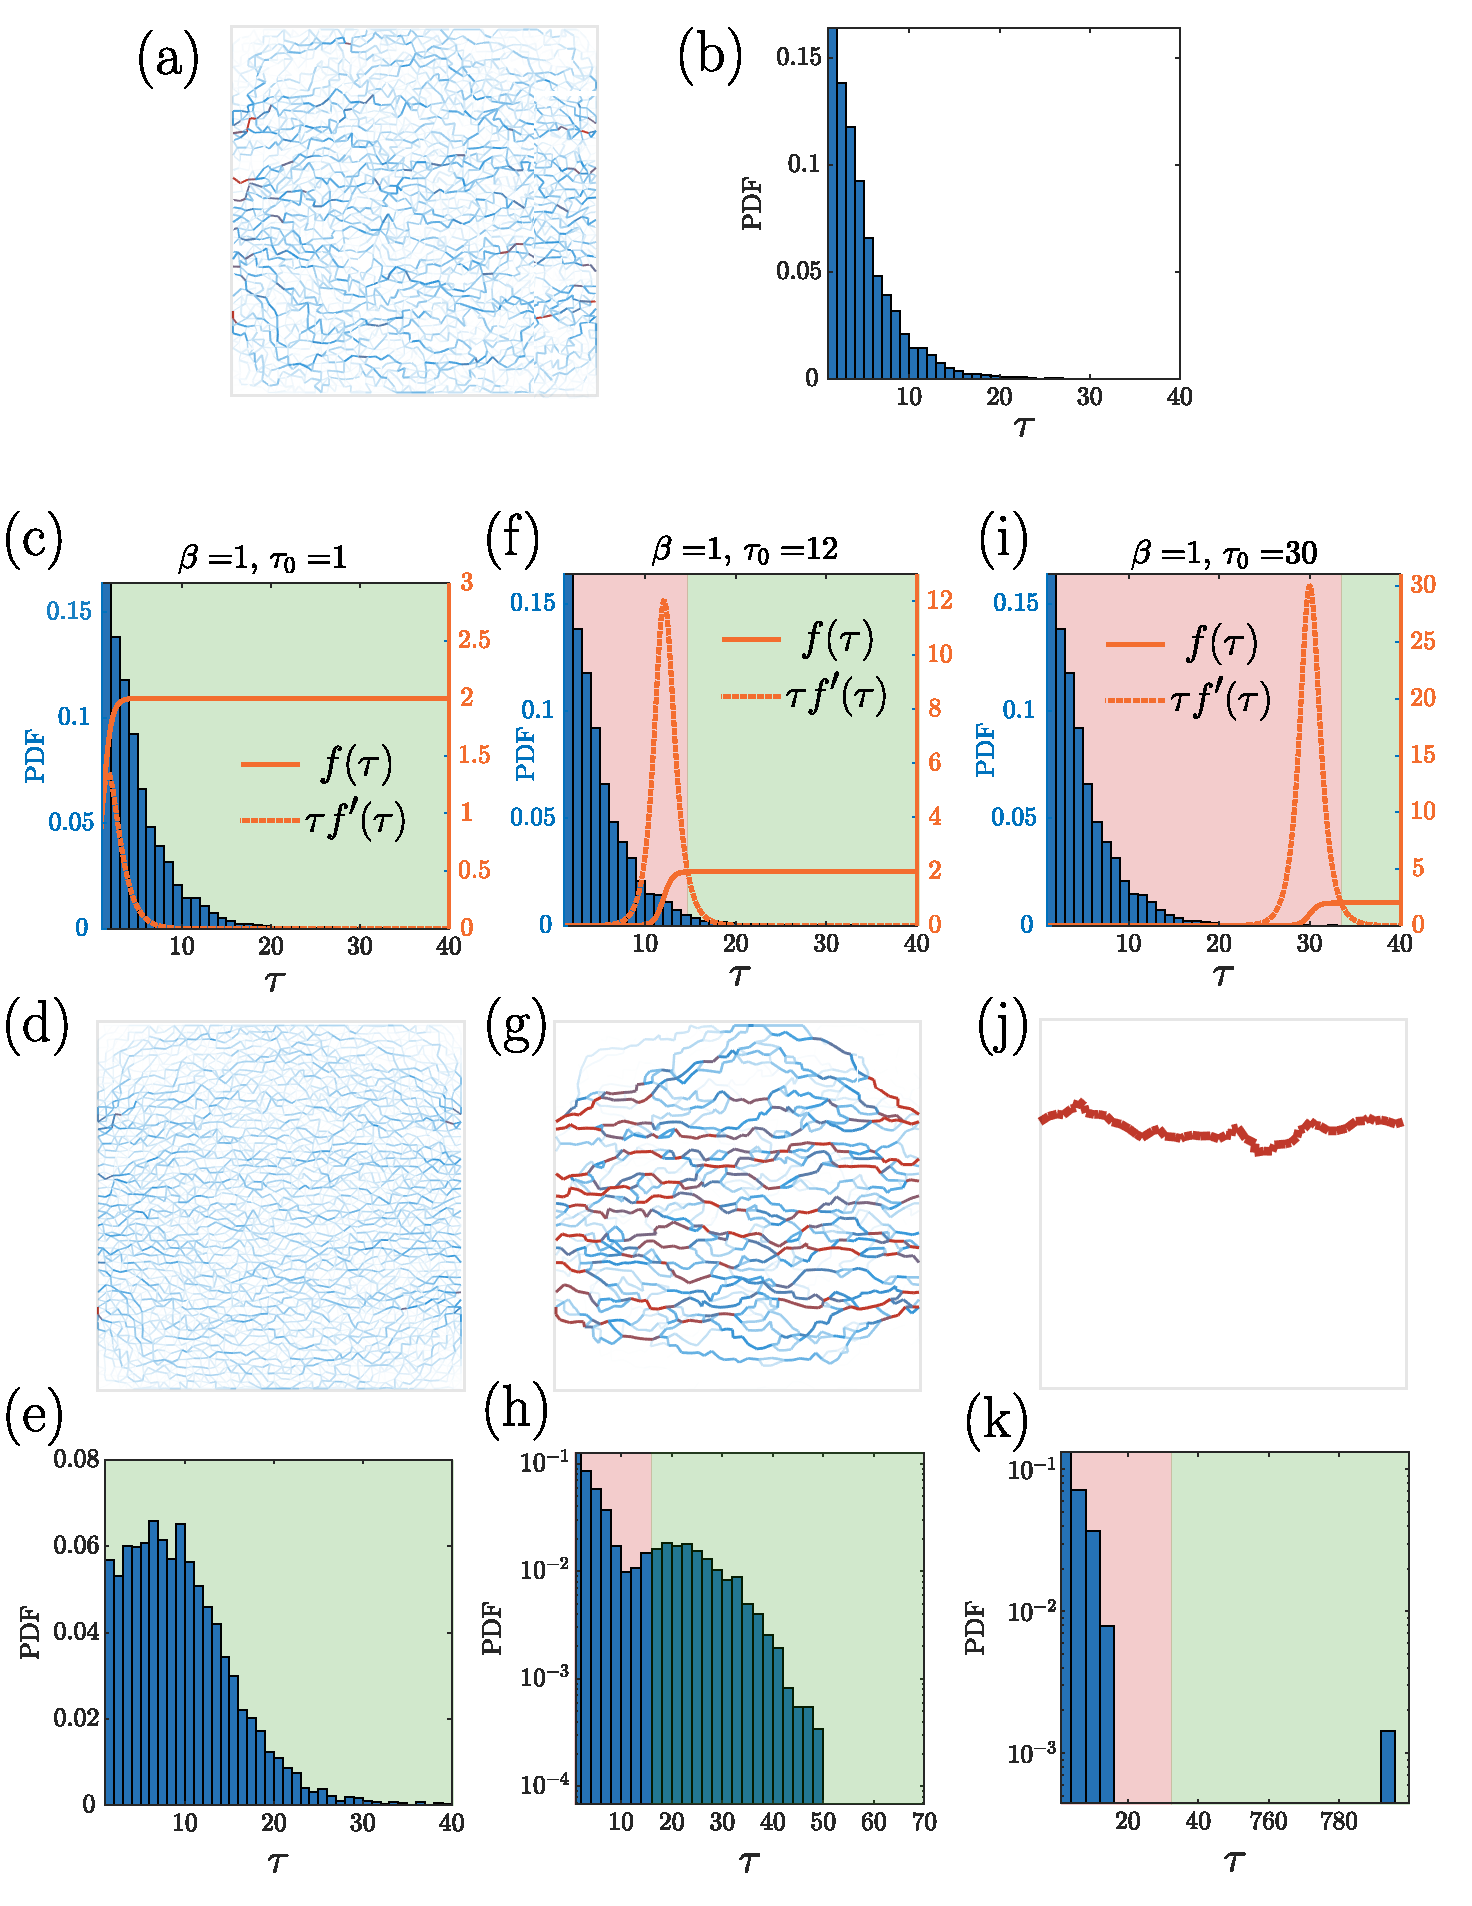
\includegraphics[width = 0.8\textwidth]{../sigmoidDelaunay.pdf}
     \caption{\textcolor{blue}{(a) A 2D random network with $N_x=50$ and $N_y=50$ points. (b) The probability distribution function (PDF) of the shear stress for the edges of the network. (c)/(f)/(i) The PDF of the shear stress along with nonlinear erosion law $f(\tau)$ (solid red line) and $\tau f'(\tau)$ (dashed red line). The areas where the homogenization condition (i.e., $f(\tau)>\tau f'(\tau)$) is satisfied are shaded with green color, otherwise, the channelization condition is satisfied and the region is shaded with red color. (d)/(g)/(j) Snapshots of the 2D network after erosion using the nonlinear erosion law shown in the previous row until the average radius of the network is increased to twice its original size. (e)/(h)/(k) The PDF of the shear stress at the walls for the final snapshot of the network shown in the previous row. 
    }}
     \label{SIfig:fig9-sigmoidDelaunay}
 \end{figure}
 \\
 
 \clearpage 



 \Answer{
     $\bullet$ (iii) From supplementary material, section S3:}
     
\AnswerQ{
\begin{quote}
In addition to the network topology and initial condition, we test the robustness of our results to changes in the boundary condition. We choose a circular domain, with the central node being the inlet and all the nodes at the outer boundary being outlets. Similar to the transition reported for the square
domain, we find a phase transition at the predicted power which shows that our analysis is independent of the geometry (Fig.~\ref{circular-S3}).
\end{quote}
}
% 
\begin{figure}[htp]
     % \centering
      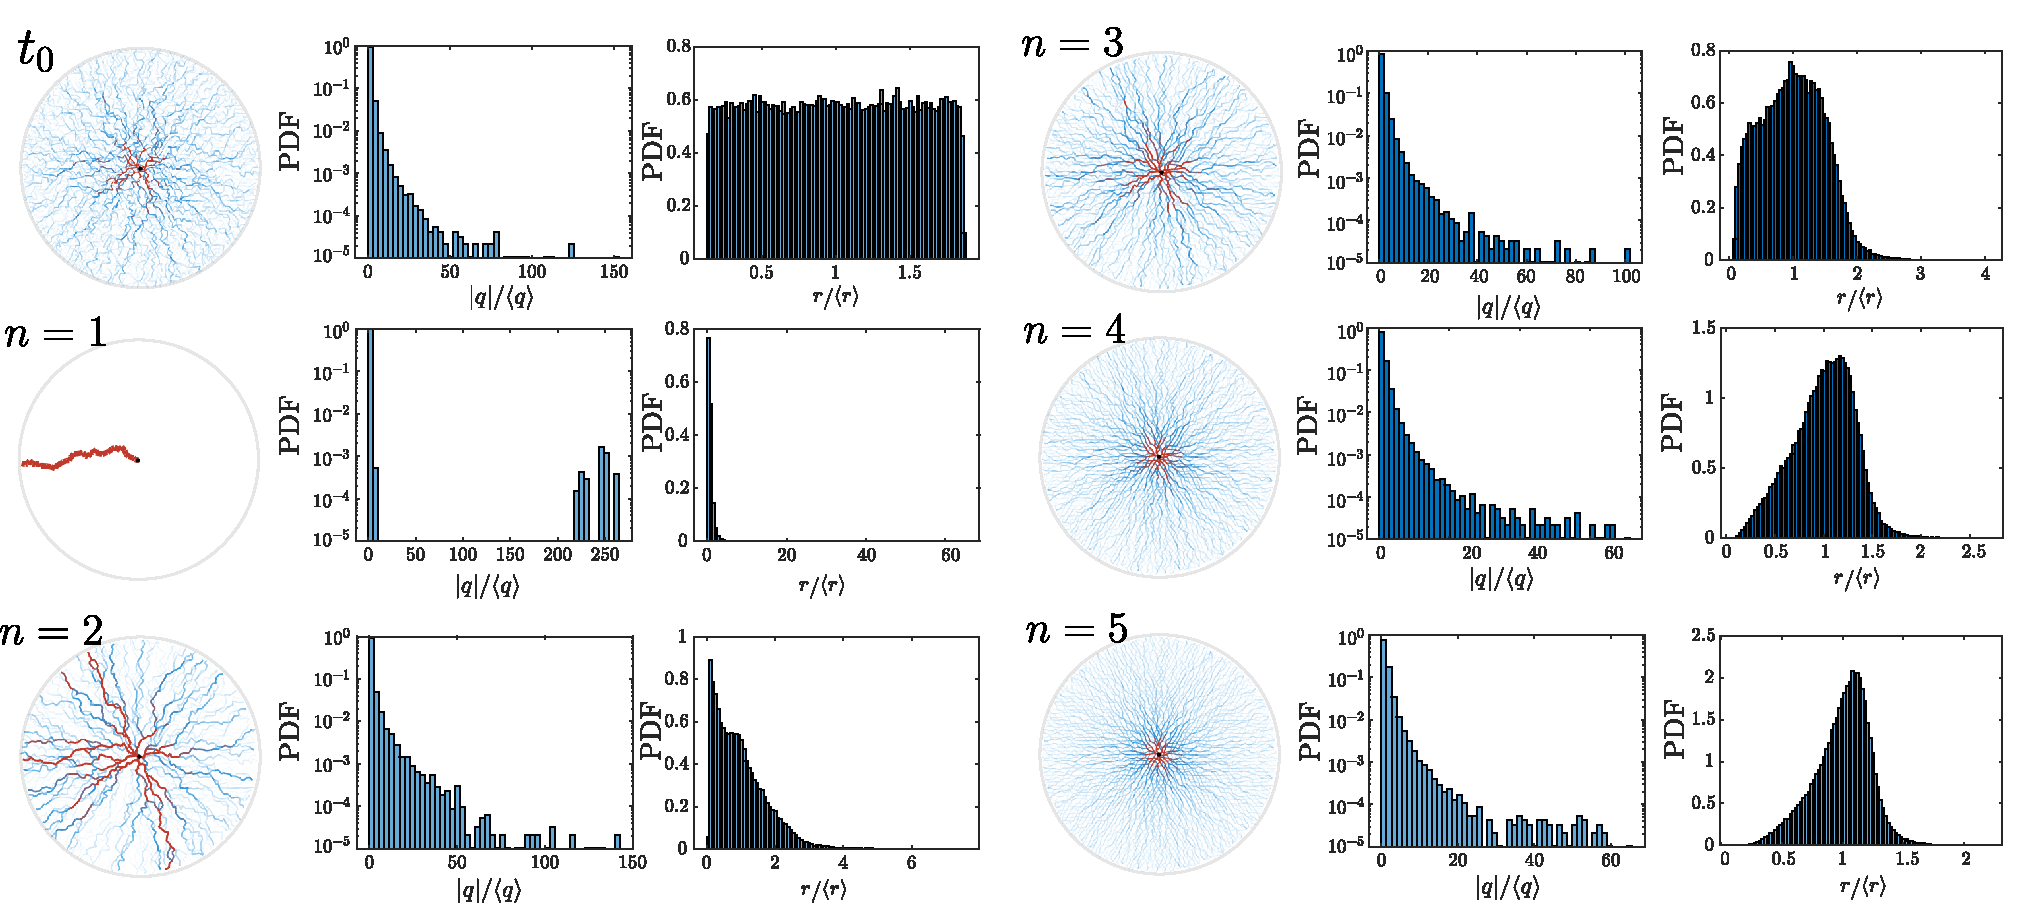
\includegraphics[width = 1.0\textwidth]{../circular.pdf}
     \caption{\add{Erosion in a topologically random 3D network of tubes with a circular topology with $N = 3000 $ randomly distributed nodes and an initial uniform broad distribution of tube diameters randomly sampled from a uniform distribution with $\mathcal{U}(1,14)$. Shown are snapshots of the network, PDF of normalized fluid flux $q/\langle q \rangle$, and normalized edge radius distribution $r/\langle r \rangle$ at the initial time $t=0$, and also after $N$ erosion steps for different powers of erosion $n$. We stop the erosion after $N$ steps such that $\langle r\rangle=2r_0$ where $r_0 = \langle r_{t=0}\rangle$. The erosion law is based on $dr/dt = \alpha q/r^n$ where different powers of $n$ correspond to different models of erosion.}}\label{circular-S3}
 \end{figure}
 
 
 \Answer{
     $\bullet$ (iv) From supplementary material, section S4:}

\AnswerQ{     
     \begin{quote}
         ``In order to make our erosion model more realistic, we modify the model as  
        %
        \begin{align}
            \frac{dr}{dt } = \begin{cases} q^m/r^n - \beta & q^m/r^n\geq \beta\\
            0 & q^m/r^n<\beta
            \end{cases} \label{eq:thresh}
        \end{align}
        %
        where $\beta$ is the threshold for the onset of erosion. We pick $\beta = 0.25\langle q^m/r^n\rangle $ and $\beta = 0.9 \langle q^m/r^n\rangle$ corresponding to a small and a large threshold value. In both cases, we ran our simulations for different values of $m$ and $n$, and found that different behaviors of homogenization and channelization persists (see Fig. \ref{fig:figthresh1}). The result can be explained by applying the general condition for the phase transition as discussed in the main text. Following the same argument, it can be shown that the homogenization condition (Eq. 3 in the main text) is equivalent to the condition 
        %
        \begin{align}
        4m-n-1 < -\frac{\beta}{q^m/r^n}.    
        \end{align}
        %
        which can be found using $g(r) = ({\pi \Delta p}/{8\mu L})^{m} r^{m-n} - \beta $ assuming a constant pressure boundary condition. Note that the condition above depends on the value of $q^m/r^n$ which varies over the network edges. Taking the mean value of $q^m/r^n$ to find an average value for the transition condition, the transition line becomes $4m-n=0.75$ and $4m-n=0.1$ for the small and large thresholding value respectively. As a result the thresholding condition slightly shifts the intercept of the transition line while the slope remains the same. In Fig.~\ref{fig:figthresh1}, we plot the new transition lines, where the prediction for the phase boundaries matches well with the simulation results.'' 
 \end{quote}
 }
 
\begin{figure}[htp]
    \centering
 \includegraphics[width=0.45\textwidth]{../Fig_thres0.25.pdf}
  \includegraphics[width=0.45\textwidth]{../Fig_thresh0.9.pdf}
     \caption{\add{Evolution of a randomly initialized network for various powers of $m$ and $n$ in Eq. \eqref{eq:thresh} with a small threshold value of $\beta = 0.25\langle q^m/r^n\rangle $ (left figure), and a large threshold value of $\beta = 0.9\langle q^m/r^n\rangle$ at $t=0$. The network is randomly initialized with $50\times 50$ randomly distributed pores. The black line shows the theoretical transition boundary between channelization instability and homogenization obtained using local dynamics model, i.e., $4m-n=0.75$ (left figure), and $4m-n=0.1$ (right figure).} }\label{fig:figthresh1}% 
\end{figure}
\\

\newpage 

\Answer{$\bullet$ (v) From \p2 of the main text:}
%

\AnswerQ{
\begin{quote}
    ``A general constitutive model for erosion can be written as $dr_{ij}/dt = f(q_{ij},r_{ij})$, where $f(q_{ij},r_{ij})$ represents the functional dependence of erosion on the fluid flux $q_{ij}$ and the tube radius $r_{ij}$. Erosion in saturated, granular, porous medium occurs when the shear stress  at the walls $\tau_w$ exerted by the fluid overcomes the cohesive strength of the solid matter $\tau_c$. In a class of erosion models previously studied~\cite{jager2017channelization,ristroph2012sculpting,wan2004investigation} the eroded mass per unit area is linearly proportional to the excess shear, i.e.,  $\dot{m}  = -\kappa  (\tau_w-\tau_c)$ where $\kappa$ is the linear proportionality constant. This erosion model effectively results in an increase in the radius of the edges in our network model where $\dot{r} \propto -\kappa r (|q|/r^3 - \tau_c)$. Similar models have further been used in biological models for the growth of vascular networks~\cite{chen2012haemodynamics,hacking1996shear}. In addition to local shear stress, erosion based on local fluid velocity ($v \propto |q|/r^2$) \cite{kudrolli2016evolution}, local pressure difference ($\Delta p \propto |q|/r^4$) \cite{derr2020flow,mahadevan2012flow}, and power dissipation ($P \propto q^2/r^4$ ) ~\cite{steeb2007modeling,marot2012study,sibille2015internal} have also been considered as alternative models. Here, we first focus on a class of erosion dynamics described by $f(q_{ij},r_{ij}) = \alpha |q_{ij}|^m/r_{ij}^n$ where $m,n,\alpha>0$ are constants. 
    This model unifies a diverse set of erosion and clogging dynamics as different values of $m$ and $n$ correspond to different physics of erosion. Later we will generalize the models to include other forms of nonlinearities.''
\end{quote}
}
\\


\Answer{We trust that these results illustrate the predictive power of the simplified model, and highlight the generality of our results.}

\newpage
%%%%%%%%%%%%%%%%%%%%%%%%%%%%%%%%%%%%%%%%%%%%%%%%%%%%%%%%%%%%%%
%%%%%%%%%%%%%%%%%%%% Review # 2
%%%%%%%%%%%%%%%%%%%%%%%%%%%%%%%%%%%%%%%%%%%%%%%%%%%%%%%%%%%

\vspace{10 mm}
\noindent
\Hline \\
\textbf{Response to Reviewer \#2} \\
\Hline
\\


\Question{This manuscript,``Temporal Evolution of Flow in Pore-Networks: From 
Homogenization to Instability'', presents a model for erosion in porous
media that treats the systems as an evolving flow network. In this
model a unique equation controls the dynamics of the radius of each
channel. The authors carry out a detailed study of the long time
dynamics of the model, identifying a phase transition depending on the
parameters of the model. The network evolves towards a
homogeneous/heterogeneous state as the control parameters cross the
critical line. The paper is sound and well written and I feel it
deserves to be published in one of the journals of the APS. However,
at the moment I am not convinced that the paper meets the necessary
criteria for publication in PRL, therefore I recommend publication in
PRE.\newline}


\Answer{We thank the reviewer for their thoughtful and thorough comments.}



\vspace{0.5cm}
\textbf{Comment 2A}
\noindent \vspace{-0.2cm}\\ \Hline\\

\Question{This paper follows other works by some of the authors regarding porous media, e.g. references [20] and [31] in the main text. I have
not been able to find a preprint of [31] what makes it difficult to
asses the potential impact of the present work. Also, since the
authors have access to experimental setups, it would greatly improve
this work if they could provide experimental proof of the phase
transition in a real system.\newline}

\Answer{We apologize for unavailability of Ref. [31]. This reference is now published and available online. The reference has been updated with publication details. With regards to the experimental tests, all the authors of the current manuscript are theorists, and experimental studies of this work is out of our scope.}
 



\vspace{0.5cm}
\textbf{Comment 2B}
\noindent \vspace{-0.2cm}\\ \Hline\\


\Question{My main concern regarding the phase transition is that I do not
know how general this effect is. For example, how would it change if
you change the boundary conditions? If all the input flow entered
through a node in the center of the network and all the boundary nodes
were sinks, conservation of mass would impose a decaying flow as you
get further apart from the center. Then equation (1) would probably
lead to a heterogeneous system even for $n>3$. Could you still
separate this behavior from the simple argument of equation (3) and
recover the phase transition? Would you have to redefine the order
parameter?\newline}


\Answer{We would like to thank the reviewer for their thoughtful comment. We have now included new numerical tests with the suggested boundary conditions. Particularly, we chose a circular domain, with the central node being the inlet and all the nodes at the outer boundary being outlets. Similar to the transition reported for the square domain, we find a phase transition at the predicted power which shows that our analysis is independent of the geometry. These new numerical simulations are now included in the supplementary material (supplementary material, Fig.~S5), see excerpt below.
Note that in our power-law model the transition depends on the relative values of $m$ and $n$, and not on the magnitude of the flux. Therefore even as one gets further from the inlet, the local criterion for the phase transition remains unchanged, in agreement with our numerical results. 

Furthermore, in the revised version we show that our results hold for a broader class of erosion models, as we expand upon in later parts of this reply.}
%
\\



 \Answer{
     $\bullet$ (iii) From supplementary material, section S3:}
     
\AnswerQ{
\begin{quote}
In addition to the network topology and initial condition, we test the robustness of our results to changes in the boundary condition. We choose a circular domain, with the central node being the inlet and all the nodes at the outer boundary being outlets. Similar to the transition reported for the square
domain, we find a phase transition at the predicted power which shows that our analysis is independent of the geometry (Fig.~\ref{circular-S3-r2}).
\end{quote}
}
% 
\begin{figure}[htp]
     % \centering
      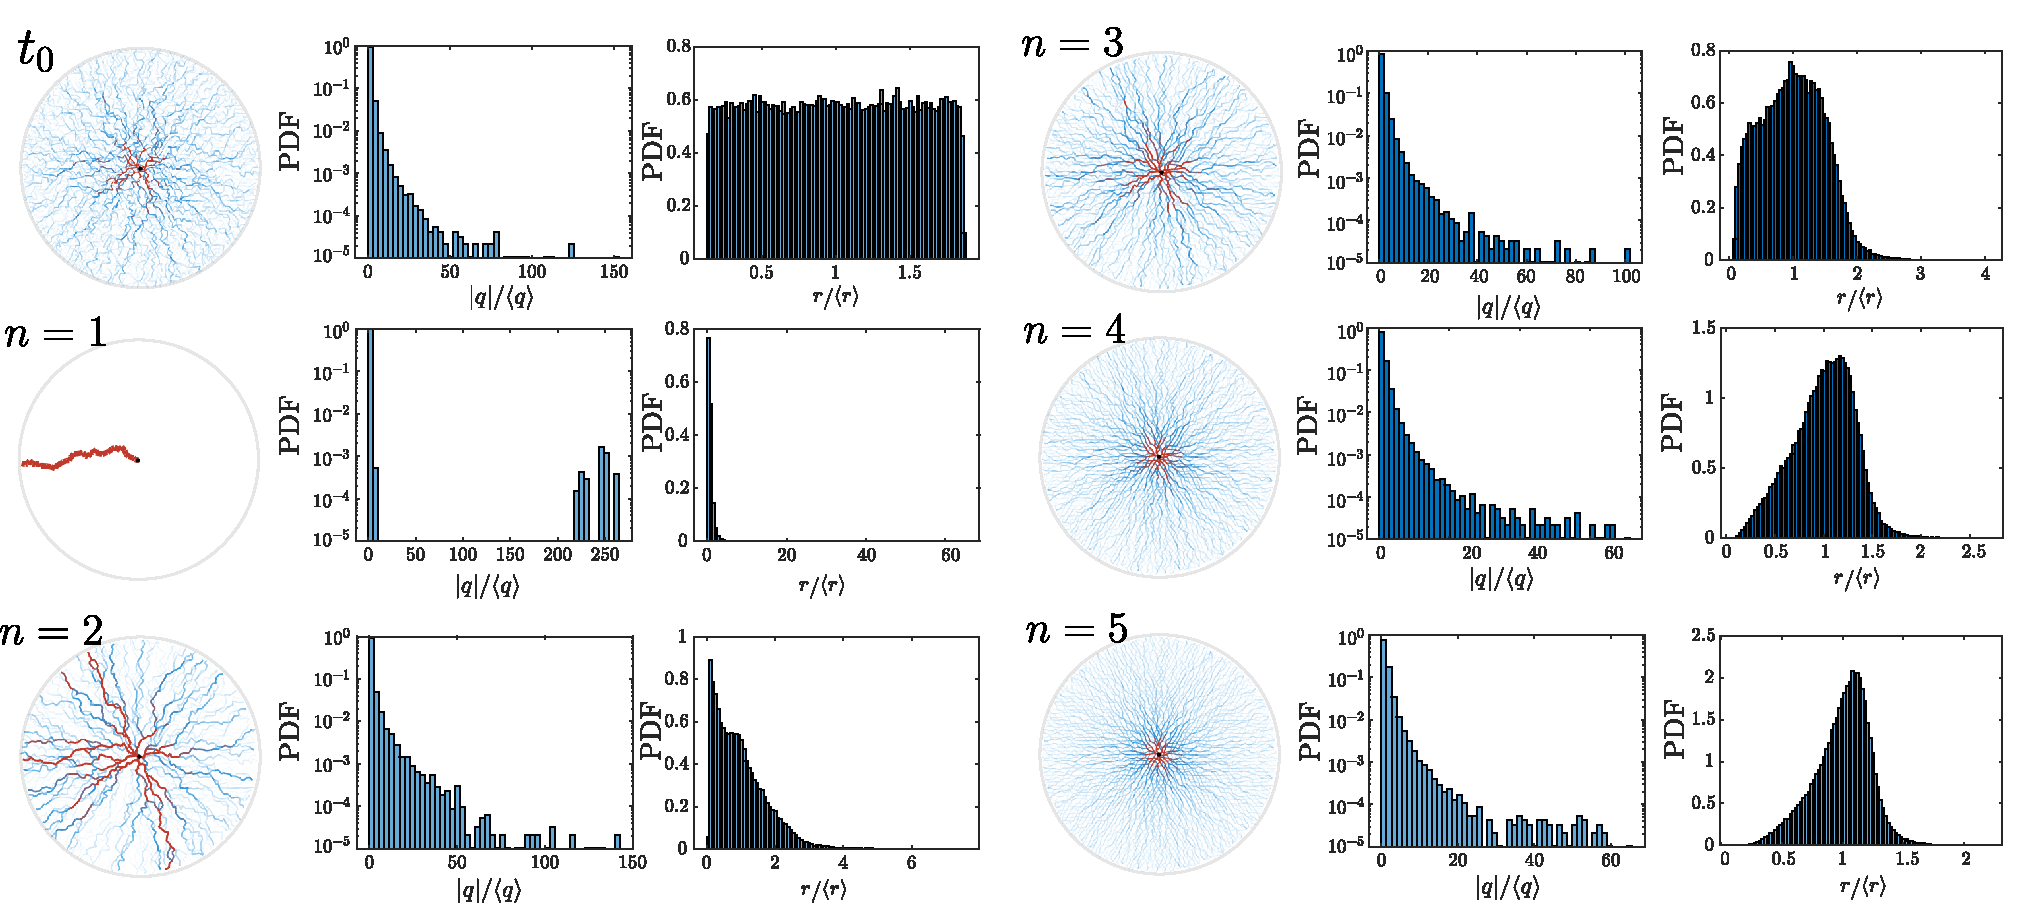
\includegraphics[width = 1.0\textwidth]{../circular.pdf}
     \caption{\add{Erosion in a topologically random 3D network of tubes with a circular topology with $N = 3000 $ randomly distributed nodes and an initial uniform broad distribution of tube diameters randomly sampled from a uniform distribution with $\mathcal{U}(1,14)$. Shown are snapshots of the network, PDF of normalized fluid flux $q/\langle q \rangle$, and normalized edge radius distribution $r/\langle r \rangle$ at the initial time $t=0$, and also after $N$ erosion steps for different powers of erosion $n$. We stop the erosion after $N$ steps such that $\langle r\rangle=2r_0$ where $r_0 = \langle r_{t=0}\rangle$. The erosion law is based on $dr/dt = \alpha q/r^n$ where different powers of $n$ correspond to different models of erosion.}}\label{circular-S3-r2}
 \end{figure}


%
    
\vspace{0.5cm}
\textbf{Comment 2C}
\noindent \vspace{-0.2cm}\\ \Hline\\

\Question{Although I agree that the order parameter defined in equation (2)
provides useful information, it could mislead the reader to think that for $n=3$ the network structure stays constant (except for some rescaling: the proportion between conductivities is conserved as argued from equation (3)). I can see ``by eye'' that the $t=0$ and the
$n=3$ panels in Fig. 2 are very different. The bigger channels align
with the flow in panel $n=3$, what makes sense from equation (1). How
does one reconcile this change in the structure with the argument
about $C_1/C_2 = cte$ for $n=3$?
\newline}

\Answer{We would like to point out that for $n=3$ the network does not stay the same, since series connections are always moving toward homogenization, while parallel connections are staying in a constant proportion. This results in seeing differences between the statistics of the network at $t=0$ and the evolved network at later stages for $n=3$ (see Fig. 2 in the main text). Additionally, we expect the transition to happen at  approximate $n\approx3$ (see comment 2G for more details). We have now included this point in the main manuscript to avoid confusion.}
%
\\

\Answer{From \p4 of the main text:}
\AnswerQ{
\begin{quote}
    ``It is to be noted that while the flow ratio remains constant for parallel edges, the connection in series are evolving toward homogenization and that is why we find a difference between evolved network for $n=3$ and the network at $t=0$.''
\end{quote}
}




\vspace{0.5cm}
\textbf{Comment 2D}
\noindent \vspace{-0.2cm}\\ \Hline\\

\Question{Could one collapse the dynamics of the authors' order parameter for
the different $n$ rescaling your time? And the PDF of the radii
rescaling the radius of the channels? In other words, if in Fig. 2. I
let the system evolve longer for $n=2$ and I rescaled all the radii
afterwards, could I get a plot ``equivalent'' to the $n=1$ case? It
would be very neat if one could show that the evolution of the system
for different $n$ and $m$ only translates to a rescaling of time and
mean radius. \newline}

\Answer{Following this comment we attempted to scale the distributions. We find that even if we rescale the probability distribution of diameters and fluid flux, the rescaled PDFs cannot be collapsed together, and depending on values of $m,n$ they follow different statistics (see Fig.~2 in the main text). We have now included the following sentence to the main text to emphasis this point.}
\\

\Answer{From \p3 of the main text:}
\AnswerQ{
\begin{quote}
    ``It is to be noted that the different distributions obtained for different powers of $m,n$ represent different statistics that cannot be collapsed.''
\end{quote}
%
}






\vspace{0.5cm}
\textbf{Comment 2E}
\noindent \vspace{-0.2cm}\\ \Hline\\

\Question{I think the model could be much richer if it tracked the solute
being eroded (through some solute concentration). That way solute
could be deposited further along the system. In that case you would
have a competing term in equation (1) including the concentration of
solute due to erosion in other parts of the system. This would lead to
a left/right asymmetry in the system of Fig. 2, and I think the system
would not tend to a homogeneous state for $n>3$.\newline}

\Answer{We thank the reviewer for their valuable. Adding solute concentration is indeed a fascinating question and a great direction for future expansion of our work. Our current approach studies erosion models with $dr/dt=f(q,r)$, however, new fields such as solute concentration, $c$, can be added to the model, $dr/dt = f(q,r,c)$, to study erosion in systems with chemical erosion. While this extension is out of our current work's scope,  we have included this point to our conclusion for future directions.}
\\

\Answer{From \p5 of the main text:}
%
\AnswerQ{
\begin{quote}
    ``Additionally, the model studied here could become richer by tracking the solute being eroded through solute concentration using $dr/dt=f(q,r,c)$ where $c$ is the solute concentration, and also allow for solute deposition further along the porous material~[53-55].''
\end{quote}
} 



\vspace{0.5cm}
\textbf{Comment 2F}
\noindent \vspace{-0.2cm}\\ \Hline\\
\Question{I think the authors should be more specific in the introduction and
name a specific system where they think their model (erosion without
deposition/sedimentation or topology changes) applies. \newline}

\Answer{Erosion in saturated granular materials occurs when the shear stress at the wall exceeds the cohesive strength of the solid matter. In the revised version, we study more realistic models with these thresholding effects, including: (i) a  model where the onset of erosion occurs only after a threshold value; (ii) a nonlinear model where erosion starts slowly after a certain threshold value and eventually saturates to a maximum value which is determined by the maximum detachment rate of particles at the pore's boundary. 
 We make predictions for both models using our analysis and find that the analytical predictions agree well with the numerical simulations. These results illustrate the generality of our model and its applicability to a diverse set of physical models. 
 
 We also expanded our introduction of the model to make a better connection with the relevant literature. In the following we attach the relevant excerpts of the main text and the supplementary material.}
 \\
 

% In a class of such erosion models, the eroded mass per
% unit area is linearly proportional to the excess shear, where it can be shown to be captured by an increase in the radius of the edges proportional to shear stress ($\tau \propto |q|/r^3$). In addition to local shear stress, erosion based on local fluid velocity ($v \propto |q|/r^2$), local pressure difference ($\Delta p \propto |q|/r^4$), and power dissipation ($P \propto q^2/r^4$) by flow have also been considered as alternative models. Here, we consider a general erosion dynamics $dr/dt = f(q,r)$, and identify the condition on $f(q,r)$ with which we can predict the fate of the network (homogenization or channelization). First, by focusing on a class of erosion dynamics $dr/dt = \alpha |q|^m/r^n$, which can capture various physics of erosion, we show different behaviors (channelization or homogenization) are possible to be observed. We then generalize the model to include a thresholding effect, and show, both analytically and numerically, how it only slightly affects the transition boundary. Finally, we test our analysis for a general erosion dynamics, by considering a nonlinear model of erosion law $dr/dt = \alpha \left( \tanh{\left[ \beta(\tau - \tau_0)\right]}+1\right)$ where $\beta$ is the shear rate scale and $\alpha$ is the erosion rate scale. In such models, 
\\
\vspace{4mm}

\Answer{$\bullet$ (i) From section S4 of the supplementary material:}
%

\AnswerQ{     
     \begin{quote}
         ``In order to make our erosion model more realistic, we modify the model as  
        %
        \begin{align}
            \frac{dr}{dt } = \begin{cases} q^m/r^n - \beta & q^m/r^n\geq \beta\\
            0 & q^m/r^n<\beta
            \end{cases} \label{eq:thresh-r2}
        \end{align}
        %
        where $\beta$ is the threshold for the onset of erosion. We pick $\beta = 0.25\langle q^m/r^n\rangle $ and $\beta = 0.9 \langle q^m/r^n\rangle$ corresponding to a small and a large threshold value. In both cases, we ran our simulations for different values of $m$ and $n$, and found that different behaviors of homogenization and channelization persists (see Fig. \ref{fig:figthresh1-r2}). The result can be explained by applying the general condition for the phase transition as discussed in the main text. Following the same argument, it can be shown that the homogenization condition (Eq. 3 in the main text) is equivalent to the condition 
        %
        \begin{align}
        4m-n-1 < -\frac{\beta}{q^m/r^n}.    
        \end{align}
        %
        which can be found using $g(r) = ({\pi \Delta p}/{8\mu L})^{m} r^{m-n} - \beta $ assuming a constant pressure boundary condition. Note that the condition above depends on the value of $q^m/r^n$ which varies over the network edges. Taking the mean value of $q^m/r^n$ to find an average value for the transition condition, the transition line becomes $4m-n=0.75$ and $4m-n=0.1$ for the small and large thresholding value respectively. As a result the thresholding condition slightly shifts the intercept of the transition line while the slope remains the same. In Fig.~\ref{fig:figthresh1-r2}, we plot the new transition lines, where the prediction for the phase boundaries matches well with the simulation results.'' 
 \end{quote}
 }
 
\begin{figure}[htp]
    \centering
 \includegraphics[width=0.45\textwidth]{../Fig_thres0.25.pdf}
  \includegraphics[width=0.45\textwidth]{../Fig_thresh0.9.pdf}
     \caption{\add{Evolution of a randomly initialized network for various powers of $m$ and $n$ in Eq. \eqref{eq:thresh-r2} with a small threshold value of $\beta = 0.25\langle q^m/r^n\rangle $ (left figure), and a large threshold value of $\beta = 0.9\langle q^m/r^n\rangle$ at $t=0$. The network is randomly initialized with $50\times 50$ randomly distributed pores. The black line shows the theoretical transition boundary between channelization instability and homogenization obtained using local dynamics model, i.e., $4m-n=0.75$ (left figure), and $4m-n=0.1$ (right figure).} }\label{fig:figthresh1-r2}% 
\end{figure}


\Answer{$\bullet$ (ii) From supplementary material, section S7:}
%

\AnswerQ{
\begin{quote}
    ``As an example of a nonlinear erosion model, we consider a shear-dependent erosion
    %
    \begin{align}
        \frac{dr}{dt} = f(\tau), 
    \end{align}
    %
    where $\tau=\tau(q,r) = 4\mu q/\pi r^3$ is the shear stress at the tube's wall assuming Poiseuille flow. It is to be noted that a shear-dependent erosion model is commonly used in studying erosion  \cite{jager2017channelization,bonelli2011micromechanical,parker2000purely} wherein such models erosion happens linearly proportional to the shear stress at the wall only after a certain threshold value $\tau_0$ (see main text for more information). Such linear models, however, ignore the maximum detachment rate of particles at the pore's boundary which would effectively limit the pore's radius maximum rate of change. To address this, we use a nonlinear erosion model
    %
    \begin{align}
        f(\tau) = \alpha \left( \tanh{\left[ \beta(\tau - \tau_0)\right]}+1\right), 
        \label{eq:sigmoidErosion-r2}
    \end{align}
    %
    where $\beta$ determines the shear rate scale and $\alpha$ determines the erosion rate scale. Note that the erosion rate scale $\alpha$ only affects the timescale at which the final state is reached and has no effect on the pattern formation. Without loss of generality we set $\alpha = 1$. Following the local dynamics model discussion in the main text, one can find that the homogenization condition reduces to 
    %
    \begin{align}
        f(\tau)>\tau \frac{df(\tau)}{d \tau}. 
        \label{eq:sigmoidCondition-r2}
    \end{align}
    %
    Assuming a random network (Fig.~\ref{SIfig:fig9-sigmoidDelaunay-r2}a), the initial values of shear stress at the walls has a  decaying distribution over a large set of values (Fig.~\ref{SIfig:fig9-sigmoidDelaunay-r2}b). 
    %Assuming nonlinear shear dependent erosion model (Eq. \eqref{eq:sigmoidErosion-r2}), and the homogenization condition (Eq. \eqref{eq:sigmoidCondition-r2}), three regions of erosion can be identified: (i) constant erosion region as $\tau\to\infty$: at this region the erosion happens at a constant rate $\lim_{\tau \to \infty} f(\tau) = 2$ and additionally the homogenization condition (Eq.~\eqref{eq:sigmoidCondition-r2}) is satisfied (since $\lim_{\tau \to \infty} f(\tau) = 2$ and $\lim_{\tau \to \infty} f'(\tau) = 0$). The homogenization results here is similar to the constant erosion rate model or $m=0,n=0$ discussed in the main text; (ii)  the slow erosion region as $\tau\to 0$. In this region both $f(\tau)$ and $\tau f'(\tau)$ are close to 0 and erosion happens at a very slow rate; (iii) the finite erosion-rate region near $\tau = \tau_0$, where $f(\tau)$ is an increasing function. In this region $\tau f'(\tau)$ has a maximum at $\beta \tau_0$ with a bandwidth of $1/\beta$. Note that here if $\beta \tau_0 < 1$, then the maximum $\tau f'(\tau)$ does not exceed 1, and the homogenization condition holds true for any $\tau$. As the value of $\tau_0$ increases, the homogenization region moves towards larger values of $\tau$ where smaller values of $\tau$ would result in channelization.  Varying $\beta$ and $\tau_0$ can change the network behavior. 
    To test our local dynamics model, we vary $\beta$ and $\tau_0$ and run three different tests: (i) $\beta=1,\tau_0=1$: For such values of $\beta,\tau$, almost all the tubes are in the homogenization region (Fig.~\ref{SIfig:fig9-sigmoidDelaunay-r2}c) and the network moves toward homogenization (Fig.~\ref{SIfig:fig9-sigmoidDelaunay-r2}d). The final PDF of the network after erosion is further shown in (Fig.~\ref{SIfig:fig9-sigmoidDelaunay-r2}e). (ii) $\beta=1, \tau_0=12$: In this case, the homogenization condition is satisfied at some finite value of shear stress $\tau_0$ where $f(\tau_0) = \tau_0 f(\tau_0)$. As a result, some edges would homogenize, and some would channelize (Fig.~\ref{SIfig:fig9-sigmoidDelaunay-r2}f). Running the simulation over a random network, we find that a finite number of channels form (Fig.~\ref{SIfig:fig9-sigmoidDelaunay-r2}g). The PDF distribution of shear stress at the wall $\tau$ correspondingly becomes bimodal (Fig.~\ref{SIfig:fig9-sigmoidDelaunay-r2}h). (iii) $\beta=1, \tau_0=30$: In this case, almost all the edges in the network are in the channelization regime  (Fig.~\ref{SIfig:fig9-sigmoidDelaunay-r2}i), and performing the simulations we find that indeed one strong single channel is formed (Fig.~\ref{SIfig:fig9-sigmoidDelaunay-r2}j) and the PDF of shear stress $\tau$ shows a clear separation between flow in the channel versus flow in the rest of the system (Fig.~\ref{SIfig:fig9-sigmoidDelaunay-r2}k).''
\end{quote}
}

   \begin{figure}[htp]
     % \centering
     \centering 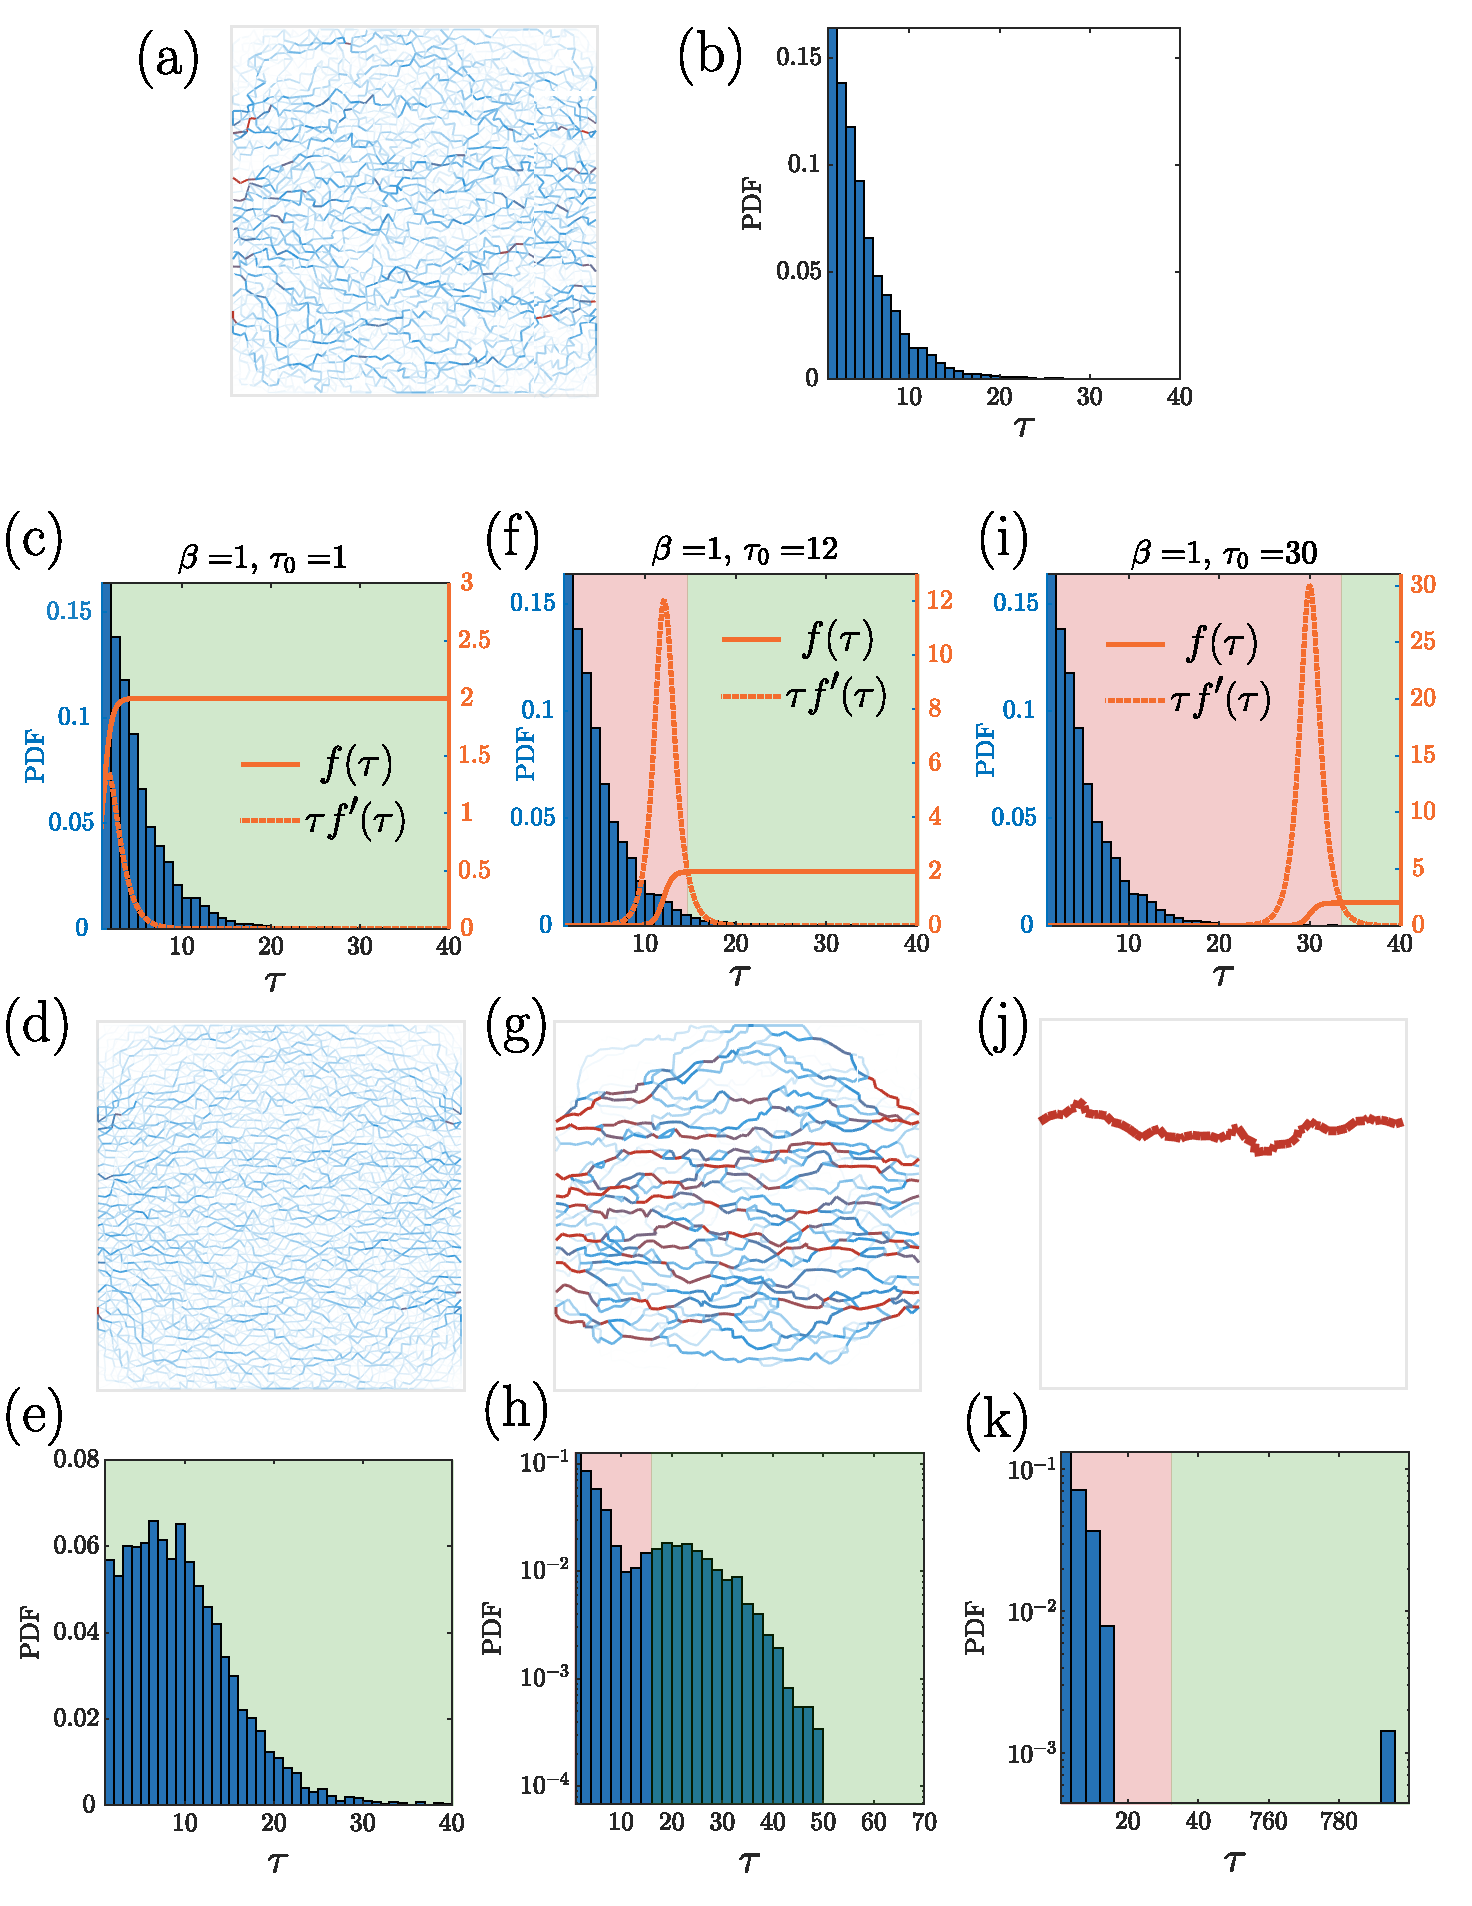
\includegraphics[width = 0.8\textwidth]{../sigmoidDelaunay.pdf}
     \caption{\textcolor{blue}{(a) A 2D random network with $N_x=50$ and $N_y=50$ points. (b) The probability distribution function (PDF) of the shear stress for the edges of the network. (c)/(f)/(i) The PDF of the shear stress along with nonlinear erosion law $f(\tau)$ (solid red line) and $\tau f'(\tau)$ (dashed red line). The areas where the homogenization condition (i.e., $f(\tau)>\tau f'(\tau)$) is satisfied are shaded with green color, otherwise, the channelization condition is satisfied and the region is shaded with red color. (d)/(g)/(j) Snapshots of the 2D network after erosion using the nonlinear erosion law shown in the previous row until the average radius of the network is increased to twice its original size. (e)/(h)/(k) The PDF of the shear stress at the walls for the final snapshot of the network shown in the previous row. 
    }}
     \label{SIfig:fig9-sigmoidDelaunay-r2}
 \end{figure}
 \\
 \clearpage 

%
\\
\vspace{4mm}

\Answer{$\bullet$ From \p3 and \p4 of the main text:}

%
\AnswerQ{
\begin{quote}
    ``\textit{Local Dynamics Model}-- \addTo understand the transition in network behavior during erosion, we focus on a simplified model with only two tubes in parallel or series with a general erosion dynamics as $dr_{i}/dt = f(q_{i},r_{i}), i=1,2$ (Figs.~3b-c). First, assuming two cylindrical tubes with radii $r_1,r_2$ in series with a given pressure difference of $\delta p = p_r- p_l$, the radius of each tube changes as $dr_i/dt = f(q,r_i),~i=1,2$ (Fig. 3b) where $q=q_1=q_2$. Without loss of generality we assume $r_1>r_2$. Considering the pressure at the junction between tubes $\tilde p_m = (p_m-p_l)/(p_r-p_l)= C_2/(C_1+C_2)$. Time evolution of the middle pressure then follows % 
    %
    \begin{align}
        \frac{d\tilde{p}_m}{dt} = \gamma (r_1 f(q,r_2)-r_2 f(q,r_1)). 
    \end{align}
    %
    where $\gamma = \sqrt{{2\pi}/{\mu L}}{C_1^{\frac{3}{4}} C_2^{\frac{3}{4}}}/{ (C_1+C_2)^2}$. In the above equation, $r_1=r_2$ is a fixed point solution where $d\tilde p_m/dt =0$ and $p_m=1/2$. Since we assumed $r_1>r_2$, we can see that $\tilde p_m <1/2$, and if ${d\tilde{p}_m}/{dt}>0$, then $\tilde p_m \to 1/2$ and the flow homogenizes. Note that if $f(q,r) = \alpha q^m/r^n$, we find that for any $n>0$ the network homogenizes (see Fig. 3b). Contrary to tubes in series, when the tubes are in parallel (Fig. 3c), the net flow $q$ divides between the two tubes in proportion to their conductivity, i.e., $ q_1/q_2 = C_1/C_2$ which results in $q_1/q = \tilde C_1$, where $\tilde C_1 = C_1/(C_1+C_2)$. Note that the dynamics for each pipe in the parallel case can be simplified to $dr_i/dt = g(r_i)$ where $g(r_i) \equiv f(q_i, r_i)$ in which $q_i = \pi r_i^4 \Delta p / 8\mu L$. Given these dynamics, the evolution of the fluid flow ratio becomes $d(q_1/q)/dt = d \tilde C_1/dt=  \gamma (r_2 g(r_1)-r_1 g(r_2))$. Similarly, it can be seen that  $r_1=r_2$ is a fixed point, where flow is equally distributed between the edges resulting in homogenization. If $d \tilde C_1/dt <0$, then the edge with larger radius has a reduced growth rate while the smaller radius edge has an increasing growth until $r_1=r_2$ is reached. This condition results in homogenization, where both edge's radius increases until the fixed point of $r_1=r_2$ is reached. The condition of $d \tilde C_1/dt<0$ is satisfied when 
    %
    \begin{align}
        \frac{g(r_1)}{g(r_2)}<\frac{r_1}{r_2}, \quad \forall r_1>r_2>0.   \label{Eq3-r2}
    \end{align}
    %
    Note that if $d\left(g(r)/r\right)/dr<0$, then Eq.~\eqref{Eq3-r2} is satisfied, and homogenization would occur.
    The above homogenization condition can further be simplified as $g(r)>g'(r)r$, which can also be obtained directly using a linear stability analysis. Given the homogenization condition $g(r)>g'(r)r$, if the erosion rate is sub-linear locally near the initial radius, the network moves towards homogenization. On the other hand, if the erosion rate is super-linear, we expect the parallel tubes to move away from homogenization and channelization occurs. Applying the power law erosion model with $f(q_{i},r_i)=\alpha q_i^m/r_i^n$, it can be shown that $g(r) \propto  r^{4m-n} $, and therefore $4m-n=1$ results in no change in the flow ratio $q_1/q$ (Fig. 3c$_1$), while $4m-n<1$ results in homogenization condition (Fig.~3c$_2$), and $4m-n>1$ results in channelization (Fig. 3c$_3$). Since a complex network includes both series and parallel connections, it is plausible that the whole network structure will behave in a similar manner, with an approximate transition in the network's behavior at $ m = (n+1)/4$. This result for $m=1$ reduces to a transition at $n=3$. It is to be noted that while the flow ratio remains constant for parallel edges, the connection in series are evolving toward homogenization and that is why we find a difference between evolved network for $n=3$ and the network at $t=0$. Since series connections are always moving toward homogenization, while parallel connections show a phase transition, we expect the phase transition to be at approximately $n\approx 3$, governed by the parallel connections. This observation  is consistent with the numerical simulation results shown in Figs.~2 and 3a (for $m=1$) as well as for additional values of $m$ (Fig.~4). Note, however, that the local dynamics model is only approximate and the numerically observed value of the phase transition happens for a value slightly larger than $n=3$ in Fig.~3. ''
    \end{quote}
}


% \Answer{We believe that the new results illustrate that the phase transition is a general effect, and our analysis using the simplified model has the predictive power of identifying the phase transition condition.}


\vspace{4mm}

\Answer{$\bullet$ From \p2 of the main text:}

%
\AnswerQ{
\begin{quote}
    ``A general constitutive model for erosion can be written as $dr_{ij}/dt = f(q_{ij},r_{ij})$, where $f(q_{ij},r_{ij})$ represents the functional dependence of erosion on the fluid flux $q_{ij}$ and the tube radius $r_{ij}$. Erosion in saturated, granular, porous medium occurs when the shear stress  at the walls $\tau_w$ exerted by the fluid overcomes the cohesive strength of the solid matter $\tau_c$. In a class of erosion models previously studied~\cite{jager2017channelization,ristroph2012sculpting,wan2004investigation} the eroded mass per unit area is linearly proportional to the excess shear, i.e.,  $\dot{m}  = -\kappa  (\tau_w-\tau_c)$ where $\kappa$ is the linear proportionality constant. This erosion model effectively results in an increase in the radius of the edges in our network model where $\dot{r} \propto -\kappa r (|q|/r^3 - \tau_c)$. Similar models have further been used in biological models for the growth of vascular networks~\cite{chen2012haemodynamics,hacking1996shear}. In addition to local shear stress, erosion based on local fluid velocity ($v \propto |q|/r^2$) \cite{kudrolli2016evolution}, local pressure difference ($\Delta p \propto |q|/r^4$) \cite{derr2020flow,mahadevan2012flow}, and power dissipation ($P \propto q^2/r^4$ ) ~\cite{steeb2007modeling,marot2012study,sibille2015internal} have also been considered as alternative models. Here, we first focus on a class of erosion dynamics described by $f(q_{ij},r_{ij}) = \alpha |q_{ij}|^m/r_{ij}^n$ where $m,n,\alpha>0$ are constants. 
    This model unifies a diverse set of erosion and clogging dynamics as different values of $m$ and $n$ correspond to different physics of erosion. Later we will generalize the models to include other forms of nonlinearities.''
\end{quote}
}



\vspace{0.5cm}
\textbf{Comment 2G}
\noindent \vspace{-0.2cm}\\ \Hline\\
\Question{Minor comment: In Fig. 3 (a) lines do not cross at exactly at $n=3$, is this correct? Do the authors have any intuition for why this
happens?\newline}

%
\\
\Answer{Indeed the transition happens at a value slightly larger than $n=3$. While the parallel connections show a phase transition at $n=3$, the series connections are always moving toward homogenization. Numerically, we expect a phase transition at $n\approx 3$ governed by the parallel connections. In the simulations, we observe a  phase transition at a value slightly larger than $n=3$. We have now included this comment in the main text.} 
\\

%consistent with the homogenization effects of the series connections
\Answer{From \p4 of the main text:}
%

\AnswerQ{\begin{quote}
    ``Since series connections are always moving toward homogenization, while parallel connections show a phase transition, we expect the phase transition to be at approximately $n\approx 3$, governed by the parallel connections. This observation  is consistent with the numerical simulation results shown in Figs.~2 and 3a (for $m=1$) as well as for additional values of $m$ (Fig.~4). Note, however, that the local dynamics model is only approximate and the numerically observed value of the phase transition happens for a value slightly larger than $n=3$ in Fig.~3.''
\end{quote}}
\\


%%%%%%%%%%%%%%%%%%%%%%%%%%%%%%%%%%%%%%%%%%%%%%%%%%%%%%%
%%%%%%%%%%%%%%%%%%%% Review # 3 %%%%%%%%%%%%%%%%%%%%%%%
%%%%%%%%%%%%%%%%%%%%%%%%%%%%%%%%%%%%%%%%%%%%%%%%%%%%%%%
\newpage 
\vspace{10 mm}
\noindent
\Hline \\
\textbf{Response to Reviewer C} \\
\Hline
\\

\Question{This paper presents 2D and 3D pore-network models of single-phase flow through porous media, involving channel erosion. The erosion rate in a channel is modeled as a function of the flow rate through the channel and the radius of the channel.The manuscript presents an interesting transition in the behaviour of these models from a stabilizing behavior where narrow channels erode more quickly than wider ones (``homogenization'') to an unstable regime where all the flow ends up in a few pathways ``instability''). Overall I judge this to be an interesting paper that may be worth publishing in a journal such as PRFluids, but falls short of the level of impact required for PRL. I explain this below.  The manuscript has many strengths which include: - it's very clearly written and with excellent figures that clearly demonstrate the phenomena being explored; - good numerical modeling that includes 2D and 3D simulations in random and regular network topologies; - results which are universal within the class of models being considered here, being valid 2D and 3D and in regular and random networks; - a clear theory to explain the results using a local analysis,suggesting links between global and local dynamics even in quite complex systems; - links to flow in biological systems
\newline}



\Answer{We thank the reviewer for their careful reading of the manuscript and their constructive
remarks.}



\vspace{0.5cm}
\textbf{Comment 3A}
\noindent \vspace{-0.2cm}\\ \Hline\\
\Question{The weaknesses in the work include: the physical relevance of the model is not clear, except for the specific biological case ... more specifics in studies of models that are closest to this one are needed, particularly also mentioning the outcomes of those studies. Some of the model's (apparent) weaknesses are being a pure power law, its scaling with pressure is unphysical: the erosion rate in all channels merely increases uniformly with applied pressure, meaning that erosion occurs even at near-zero speed/stress; there is no onset threshold.\newline}

\Answer{We appreciate the reviewers comment. The concern here is similar to comment 2F of Reviewer 2, and we repeat our reply here. Erosion in saturated granular materials occurs when the shear stress at the wall exceeds the cohesive strength of the solid matter. In the revised version, we study more realistic models including: (i) a model where the onset of erosion happens after reaching a threshold value; (ii) a model with a different (nonlinear) functional dependence on shear stress, where erosion starts after a certain threshold and eventually saturates to a maximum value which is determined by the maximal detachment rate of particles at the tube's boundary. We make predictions for both models using our analysis and find that the analytical results agree well with the numerical simulations. These results illustrate the generality of our model in relating to various physical models. (iii) Additionally, we expand our discussion before introducing the model to make a better connection with relevant studies of erosion. 
We believe that these new results illustrate that the phase transition is a general effect, and that our analysis using the local dynamics model has the predictive power of identifying the phase transition condition. In the following we attach the relevant excerpts of the main text and the supplementary material.}
\\

\vspace{4mm}

\Answer{$\bullet$ (i) From section S4 of the supplementary material:}
%

\AnswerQ{     
     \begin{quote}
         ``In order to make our erosion model more realistic, we modify the model as  
        %
        \begin{align}
            \frac{dr}{dt } = \begin{cases} q^m/r^n - \beta & q^m/r^n\geq \beta\\
            0 & q^m/r^n<\beta
            \end{cases} \label{eq:thresh-r3}
        \end{align}
        %
        where $\beta$ is the threshold for the onset of erosion. We pick $\beta = 0.25\langle q^m/r^n\rangle $ and $\beta = 0.9 \langle q^m/r^n\rangle$ corresponding to a small and a large threshold value. In both cases, we ran our simulations for different values of $m$ and $n$, and found that different behaviors of homogenization and channelization persists (see Fig. \ref{fig:figthresh1-r3}). The result can be explained by applying the general condition for the phase transition as discussed in the main text. Following the same argument, it can be shown that the homogenization condition (Eq. 3 in the main text) is equivalent to the condition 
        %
        \begin{align}
        4m-n-1 < -\frac{\beta}{q^m/r^n}.    
        \end{align}
        %
        which can be found using $g(r) = ({\pi \Delta p}/{8\mu L})^{m} r^{m-n} - \beta $ assuming a constant pressure boundary condition. Note that the condition above depends on the value of $q^m/r^n$ which varies over the network edges. Taking the mean value of $q^m/r^n$ to find an average value for the transition condition, the transition line becomes $4m-n=0.75$ and $4m-n=0.1$ for the small and large thresholding value respectively. As a result the thresholding condition slightly shifts the intercept of the transition line while the slope remains the same. In Fig.~\ref{fig:figthresh1-r3}, we plot the new transition lines, where the prediction for the phase boundaries matches well with the simulation results.'' 
 \end{quote}
 }
 
\begin{figure}[htp]
    \centering
 \includegraphics[width=0.45\textwidth]{../Fig_thres0.25.pdf}
  \includegraphics[width=0.45\textwidth]{../Fig_thresh0.9.pdf}
     \caption{\add{Evolution of a randomly initialized network for various powers of $m$ and $n$ in Eq. \eqref{eq:thresh-r3} with a small threshold value of $\beta = 0.25\langle q^m/r^n\rangle $ (left figure), and a large threshold value of $\beta = 0.9\langle q^m/r^n\rangle$ at $t=0$. The network is randomly initialized with $50\times 50$ randomly distributed pores. The black line shows the theoretical transition boundary between channelization instability and homogenization obtained using local dynamics model, i.e., $4m-n=0.75$ (left figure), and $4m-n=0.1$ (right figure).} }\label{fig:figthresh1-r3}% 
\end{figure}
%
\\
\vspace{4mm}


\Answer{$\bullet$ (ii) From supplementary material, section S7:}
%

\AnswerQ{
\begin{quote}
    ``As an example of a nonlinear erosion model, we consider a shear-dependent erosion
    %
    \begin{align}
        \frac{dr}{dt} = f(\tau), 
    \end{align}
    %
    where $\tau=\tau(q,r) = 4\mu q/\pi r^3$ is the shear stress at the tube's wall assuming Poiseuille flow. It is to be noted that a shear-dependent erosion model is commonly used in studying erosion  \cite{jager2017channelization,bonelli2011micromechanical,parker2000purely} wherein such models erosion happens linearly proportional to the shear stress at the wall only after a certain threshold value $\tau_0$ (see main text for more information). Such linear models, however, ignore the maximum detachment rate of particles at the pore's boundary which would effectively limit the pore's radius maximum rate of change. To address this, we use a nonlinear erosion model
    %
    \begin{align}
        f(\tau) = \alpha \left( \tanh{\left[ \beta(\tau - \tau_0)\right]}+1\right), 
        \label{eq:sigmoidErosion-r3}
    \end{align}
    %
    where $\beta$ determines the shear rate scale and $\alpha$ determines the erosion rate scale. Note that the erosion rate scale $\alpha$ only affects the timescale at which the final state is reached and has no effect on the pattern formation. Without loss of generality we set $\alpha = 1$. Following the local dynamics model discussion in the main text, one can find that the homogenization condition reduces to 
    %
    \begin{align}
        f(\tau)>\tau \frac{df(\tau)}{d \tau}. 
        \label{eq:sigmoidCondition-r3}
    \end{align}
    %
    Assuming a random network (Fig.~\ref{SIfig:fig9-sigmoidDelaunay-r3}a), the initial values of shear stress at the walls has a  decaying distribution over a large set of values (Fig.~\ref{SIfig:fig9-sigmoidDelaunay-r3}b). 
    %Assuming nonlinear shear dependent erosion model (Eq. \eqref{eq:sigmoidErosion-r2}), and the homogenization condition (Eq. \eqref{eq:sigmoidCondition-r3}), three regions of erosion can be identified: (i) constant erosion region as $\tau\to\infty$: at this region the erosion happens at a constant rate $\lim_{\tau \to \infty} f(\tau) = 2$ and additionally the homogenization condition (Eq.~\eqref{eq:sigmoidCondition-r3}) is satisfied (since $\lim_{\tau \to \infty} f(\tau) = 2$ and $\lim_{\tau \to \infty} f'(\tau) = 0$). The homogenization results here is similar to the constant erosion rate model or $m=0,n=0$ discussed in the main text; (ii)  the slow erosion region as $\tau\to 0$. In this region both $f(\tau)$ and $\tau f'(\tau)$ are close to 0 and erosion happens at a very slow rate; (iii) the finite erosion-rate region near $\tau = \tau_0$, where $f(\tau)$ is an increasing function. In this region $\tau f'(\tau)$ has a maximum at $\beta \tau_0$ with a bandwidth of $1/\beta$. Note that here if $\beta \tau_0 < 1$, then the maximum $\tau f'(\tau)$ does not exceed 1, and the homogenization condition holds true for any $\tau$. As the value of $\tau_0$ increases, the homogenization region moves towards larger values of $\tau$ where smaller values of $\tau$ would result in channelization.  Varying $\beta$ and $\tau_0$ can change the network behavior. 
    To test our local dynamics model, we vary $\beta$ and $\tau_0$ and run three different tests: (i) $\beta=1,\tau_0=1$: For such values of $\beta,\tau$, almost all the tubes are in the homogenization region (Fig.~\ref{SIfig:fig9-sigmoidDelaunay-r3}c) and the network moves toward homogenization (Fig.~\ref{SIfig:fig9-sigmoidDelaunay-r3}d). The final PDF of the network after erosion is further shown in (Fig.~\ref{SIfig:fig9-sigmoidDelaunay-r3}e). (ii) $\beta=1, \tau_0=12$: In this case, the homogenization condition is satisfied at some finite value of shear stress $\tau_0$ where $f(\tau_0) = \tau_0 f(\tau_0)$. As a result, some edges would homogenize, and some would channelize (Fig.~\ref{SIfig:fig9-sigmoidDelaunay-r3}f). Running the simulation over a random network, we find that a finite number of channels form (Fig.~\ref{SIfig:fig9-sigmoidDelaunay-r3}g). The PDF distribution of shear stress at the wall $\tau$ correspondingly becomes bimodal (Fig.~\ref{SIfig:fig9-sigmoidDelaunay-r3}h). (iii) $\beta=1, \tau_0=30$: In this case, almost all the edges in the network are in the channelization regime  (Fig.~\ref{SIfig:fig9-sigmoidDelaunay-r3}i), and performing the simulations we find that indeed one strong single channel is formed (Fig.~\ref{SIfig:fig9-sigmoidDelaunay-r3}j) and the PDF of shear stress $\tau$ shows a clear separation between flow in the channel versus flow in the rest of the system (Fig.~\ref{SIfig:fig9-sigmoidDelaunay-r3}k).''
\end{quote}
}

   \begin{figure}[htp]
     % \centering
     \centering 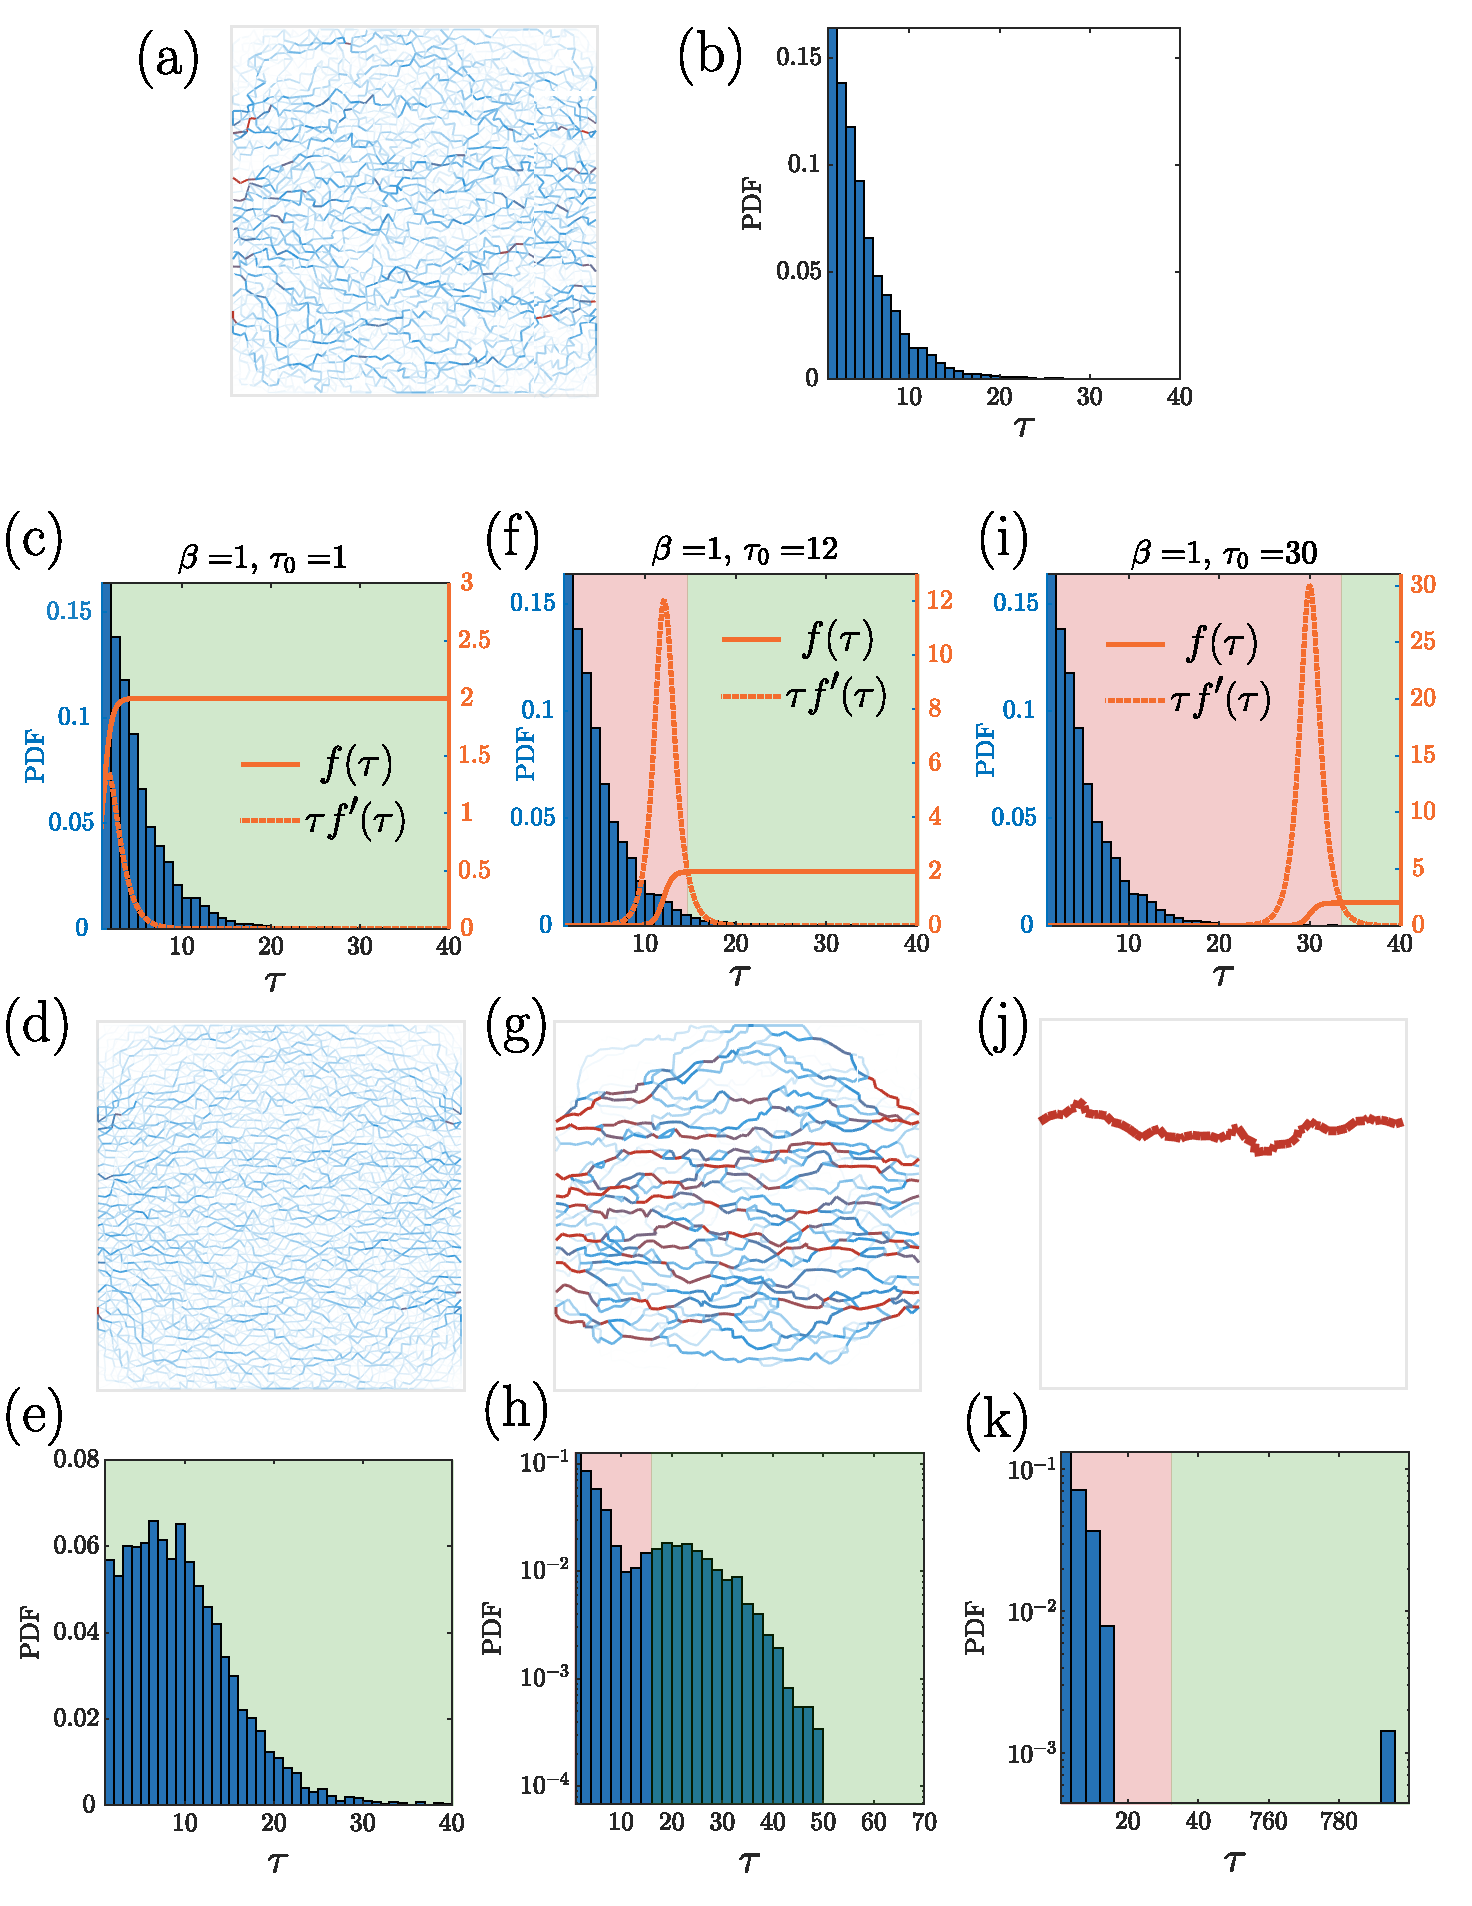
\includegraphics[width = 0.8\textwidth]{../sigmoidDelaunay.pdf}
     \caption{\textcolor{blue}{(a) A 2D random network with $N_x=50$ and $N_y=50$ points. (b) The probability distribution function (PDF) of the shear stress for the edges of the network. (c)/(f)/(i) The PDF of the shear stress along with nonlinear erosion law $f(\tau)$ (solid red line) and $\tau f'(\tau)$ (dashed red line). The areas where the homogenization condition (i.e., $f(\tau)>\tau f'(\tau)$) is satisfied are shaded with green color, otherwise, the channelization condition is satisfied and the region is shaded with red color. (d)/(g)/(j) Snapshots of the 2D network after erosion using the nonlinear erosion law shown in the previous row until the average radius of the network is increased to twice its original size. (e)/(h)/(k) The PDF of the shear stress at the walls for the final snapshot of the network shown in the previous row. 
    }}
     \label{SIfig:fig9-sigmoidDelaunay-r3}
 \end{figure}

\clearpage 


\Answer{$\bullet$ (iii) From \p2 of the main text:}

\AnswerQ{
\begin{quote}
    ``A general constitutive model for erosion can be written as $dr_{ij}/dt = f(q_{ij},r_{ij})$, where $f(q_{ij},r_{ij})$ represents the functional dependence of erosion on the fluid flux $q_{ij}$ and the tube radius $r_{ij}$. Erosion in saturated, granular, porous medium occurs when the shear stress  at the walls $\tau_w$ exerted by the fluid overcomes the cohesive strength of the solid matter $\tau_c$. In a class of erosion models previously studied~\cite{jager2017channelization,ristroph2012sculpting,wan2004investigation} the eroded mass per unit area is linearly proportional to the excess shear, i.e.,  $\dot{m}  = -\kappa  (\tau_w-\tau_c)$ where $\kappa$ is the linear proportionality constant. This erosion model effectively results in an increase in the radius of the edges in our network model where $\dot{r} \propto -\kappa r (|q|/r^3 - \tau_c)$. Similar models have further been used in biological models for the growth of vascular networks~\cite{chen2012haemodynamics,hacking1996shear}. In addition to local shear stress, erosion based on local fluid velocity ($v \propto |q|/r^2$) \cite{kudrolli2016evolution}, local pressure difference ($\Delta p \propto |q|/r^4$) \cite{derr2020flow,mahadevan2012flow}, and power dissipation ($P \propto q^2/r^4$ ) ~\cite{steeb2007modeling,marot2012study,sibille2015internal} have also been considered as alternative models. Here, we first focus on a class of erosion dynamics described by $f(q_{ij},r_{ij}) = \alpha |q_{ij}|^m/r_{ij}^n$ where $m,n,\alpha>0$ are constants. 
    This model unifies a diverse set of erosion and clogging dynamics as different values of $m$ and $n$ correspond to different physics of erosion. Later we will generalize the models to include other forms of nonlinearities.''
\end{quote}
}



% \Answer{We believe that the new results illustrate that the phase transition is a general effect, and our analysis using the simplified model has the predictive power of identifying the phase transition condition.}



% \newpage
% \vspace{0.5cm}
% \textbf{Comment 3B}
% \noindent \vspace{-0.2cm}\\ \Hline\\
% \Question{\newline}

% \Answer{To address this point, we ran new numerical simulations with thresholding effect. Particularly, we add a threshold value $\beta$ for the onset of erosion to our dynamics. We pick a small and a large value for the onset of erosion $\beta$. In both cases, we ran our experiments for different values of $m$ and $n$, and we find that the model transition line stay at $n=(m+1)/4$ and does not change (see comment 3A and Fig. \ref{fig:figthresh22}). The new threshhold model and simulations are included in the supplementary material with a reference to them in the main text. In addition to the threshold model, we consider a more realistic nonlinear model for erosion $dr/dt = \alpha \left( \tanh{\left[ \beta(\tau - \tau_0)\right]}+1\right)$ where $\beta$ determines the shear rate scale and $\alpha$ determines the erosion rate scale. In this erosion model, erosion starts slowly after a certain threshold and eventually saturates to a maximum value which is determined by the maximum detachment rate of particles at the pore's boundary. We make predictions with our analysis and find that our approach matches with the numerical simulations. These results proves the generality of our model in predicting the fate of the network for various physical models that are considered in literature. In the following we attach the relevant excerpts of the main text and the supplementary material.
% }
% \\


\vspace{0.5cm}
\textbf{Comment 3B}
\noindent \vspace{-0.2cm}\\ \Hline\\
\Question{ the existence of a homogenisation regime is surely unphysical, since this regime only occurs in cases where erosion is inversely dependent on fluid velocity - the manuscript's use of flow rate rather
than velocity slightly obscures this fact.
\newline}

\Answer{We thank the reviewer for their comment. The regime corresponding to homogenization corresponds to cases with $m<(n+1)/4$, an example of which would be an erosion proportional to local fluid velocity $dr/dt \propto q/r^2$. We have rephrased the relevant sentence to make this point clear. Additionally, we would like to point out that the homogenization regime correspond to a family of models and erosion proportional to velocity is \emph{e pluribus unum}. In the revised manuscript, we have generalized our model, and found the condition for homogenization within a general class of erosion models following the dynamics $dr/dt=f(q,r)$, see the relevant excerpt from the revised main text attached below.}
\vspace{4mm}


\Answer{$\bullet$ From \p3 and \p4 of the main text:}
%

\AnswerQ{
\begin{quote}
    ``\textit{Local Dynamics Model}-- To understand the transition in network behavior during erosion, we focus on a simplified model with only two tubes in parallel or series with a general erosion dynamics as $dr_{i}/dt = f(q_{i},r_{i}), i=1,2$ (Figs.~3b-c). First, assuming two cylindrical tubes with radii $r_1,r_2$ in series with a given pressure difference of $\delta p = p_r- p_l$, the radius of each tube changes as $dr_i/dt = f(q,r_i),~i=1,2$ (Fig. 3b) where $q=q_1=q_2$. Without loss of generality we assume $r_1>r_2$. Considering the pressure at the junction between tubes $\tilde p_m = (p_m-p_l)/(p_r-p_l)= C_2/(C_1+C_2)$. Time evolution of the middle pressure then follows % 
    %
    \begin{align}
        \frac{d\tilde{p}_m}{dt} = \gamma (r_1 f(q,r_2)-r_2 f(q,r_1)). 
    \end{align}
    %
    where $\gamma = \sqrt{{2\pi}/{\mu L}}{C_1^{\frac{3}{4}} C_2^{\frac{3}{4}}}/{ (C_1+C_2)^2}$. In the above equation, $r_1=r_2$ is a fixed point solution where $d\tilde p_m/dt =0$ and $p_m=1/2$. Since we assumed $r_1>r_2$, we can see that $\tilde p_m <1/2$, and if ${d\tilde{p}_m}/{dt}>0$, then $\tilde p_m \to 1/2$ and the flow homogenizes. Note that if $f(q,r) = \alpha q^m/r^n$, we find that for any $n>0$ the network homogenizes (see Fig. 3b). Contrary to tubes in series, when the tubes are in parallel (Fig. 3c), the net flow $q$ divides between the two tubes in proportion to their conductivity, i.e., $ q_1/q_2 = C_1/C_2$ which results in $q_1/q = \tilde C_1$, where $\tilde C_1 = C_1/(C_1+C_2)$. Note that the dynamics for each pipe in the parallel case can be simplified to $dr_i/dt = g(r_i)$ where $g(r_i) \equiv f(q_i, r_i)$ in which $q_i = \pi r_i^4 \Delta p / 8\mu L$. Given these dynamics, the evolution of the fluid flow ratio becomes $d(q_1/q)/dt = d \tilde C_1/dt=  \gamma (r_2 g(r_1)-r_1 g(r_2))$. Similarly, it can be seen that  $r_1=r_2$ is a fixed point, where flow is equally distributed between the edges resulting in homogenization. If $d \tilde C_1/dt <0$, then the edge with larger radius has a reduced growth rate while the smaller radius edge has an increasing growth until $r_1=r_2$ is reached. This condition results in homogenization, where both edge's radius increases until the fixed point of $r_1=r_2$ is reached. The condition of $d \tilde C_1/dt<0$ is satisfied when 
    %
    \begin{align}
        \frac{g(r_1)}{g(r_2)}<\frac{r_1}{r_2}, \quad \forall r_1>r_2>0.   \label{Eq3-r3}
    \end{align}
    %
    Note that if $d\left(g(r)/r\right)/dr<0$, then Eq.~\eqref{Eq3-r3} is satisfied, and homogenization would occur.
    The above homogenization condition can further be simplified as $g(r)>g'(r)r$, which can also be obtained directly using a linear stability analysis. Given the homogenization condition $g(r)>g'(r)r$, if the erosion rate is sub-linear locally near the initial radius, the network moves towards homogenization. On the other hand, if the erosion rate is super-linear, we expect the parallel tubes to move away from homogenization and channelization occurs. Applying the power law erosion model with $f(q_{i},r_i)=\alpha q_i^m/r_i^n$, it can be shown that $g(r) \propto  r^{4m-n} $, and therefore $4m-n=1$ results in no change in the flow ratio $q_1/q$ (Fig. 3c$_1$), while $4m-n<1$ results in homogenization condition (Fig.~3c$_2$), and $4m-n>1$ results in channelization (Fig. 3c$_3$). Since a complex network includes both series and parallel connections, it is plausible that the whole network structure will behave in a similar manner, with an approximate transition in the network's behavior at $ m = (n+1)/4$. This result for $m=1$ reduces to a transition at $n=3$. It is to be noted that while the flow ratio remains constant for parallel edges, the connections in series are evolving toward homogenization and that is why we find a difference between evolved network for $n=3$ and the network at $t=0$. Since series connections are always moving toward homogenization, while parallel connections show a phase transition, we expect the phase transition to be at approximately $n\approx 3$, governed by the parallel connections. This observation  is consistent with the numerical simulation results shown in Figs.~2 and 3a (for $m=1$) as well as for additional values of $m$ (Fig.~4). Note, however, that the local dynamics model is only approximate and the numerically observed value of the phase transition happens for a value slightly larger than $n=3$ in Fig.~3.''
    \end{quote}
}



\vspace{0.5cm}
\textbf{Comment 3C}
\noindent \vspace{-0.2cm}\\ \Hline\\
\Question{The model almost seems contrived to exhibit a stability transition, ... The authors appear to have chosen a model based on the ease of analysis, and uncovered a clear and rather universal transition in this model's behavior. However the model lacks fundamental aspects of erosion physics (such as an erosion-onset threshold) and yields a scaling on channel diameter that is too similar to Poiseuille's law for flow. The universal transition in the model appears to a relatively unsurprising consequence of this similarity, and one imagines that the universality would disappear if the model were changed even slightly. It is also unclear whether a homogenization regime would exist at all in any but the most contrived physical
systems.\newline}

\Answer{As mentioned above, in the revised version we have considered a general erosion law $dr/dt=f(q,r)$ and identified the stability condition for the homogeneous phase.  Additionally, as mentioned in our reply to the first comment we significantly extended our analysis to a broad range of models incoporating different forms of nonlinearities. We find that our approach correctly predicts the onset of channeling and the fate of network (see comment 3A). }
\\


\vspace{0.5cm}
\textbf{Comment 3D}
\noindent \vspace{-0.2cm}\\ \Hline\\
\Question{minimal discussion of experimental results. One set of relevant
results is the transition to wormhole formation that occurs in
carbonic acid flow through limestone formations. The authors may feel
that the erosion studied here is distinct from reactive flow but the
similarities are highly significant. I advise the authors to investigate the reactive transport
literature in more depth. In terms of wormhole formation here is one
publication among many: Ott and Oedai GRL 2016 \\ 
https://doi.org/10.1002/2015GL063582.
\newline}


\Answer{We thank the reviewer for bringing this article to our attention. Since it is very relevant to our study and our model can potentially be expanded to study geologically studies, we have included it in our conclusion for future directions. The relevant part is attached in the following.}
\\

\Answer{$\bullet$ From \p5 of the main text:}
%

\AnswerQ{
\begin{quote}
    ``In the future, it would be exciting to test this and other predictions experimentally on model systems, relying on the technological advances in imaging flow profiles in porous materials, as well as extend the study to the geologically relevant case of chemical erosion \cite{edery2014origins,edery2016characterization}, and wormhole formation in geologic formations during CO$_2$ injection \cite{ott2015wormhole,szymczak2009wormhole}. Additionally, the model studied here could become richer by tracking the solute being eroded through solute concentration using $dr/dt=f(q,r,c)$ where $c$ is the solute concentration, and allow for solute deposition along the porous material~\cite{bizmark2020multiscale,jager2018clogging,jaeger2017mechanism}.''
\end{quote}

}

% \vspace{0.5cm}
% \textbf{Comment 3G}
% \noindent \vspace{-0.2cm}\\ \Hline\\
% \Question{When the strengths and weakness are considered together it is clear that this work does not have the level of impact expected for PRL, particularly when judged against the weaknesses. The work looks suitable for a different journal if there is some addressal of the weaknesses described above.
% \newline}

% \Answer{...   }



% \vspace{0.5cm}
% \textbf{Comment 3H}
% \noindent \vspace{-0.2cm}\\ \Hline\\
% \Question{The authors appear to have chosen a model based on the ease of analysis, and uncovered a clear and rather universal transition in this model's behavior. However the model lacks fundamental aspects of erosion physics (such as an erosion-onset threshold) and yields a scaling on channel diameter that is too similar to Poiseuille's law for flow. The universal transition in the model appears to a relatively unsurprising consequence of this similarity, and one imagines that the universality would disappear if the model were changed even slightly. It is also unclear whether a homogenization regime would exist at all in any but the most contrived physical
% systems..\newline}

% \Answer{In order to address this issue, we ran new numerical experiments to check for the (a) effect of different boundary conditions (see comment 2B), and also (b) adding a threshold for the onset of erosion (see comment 3C), where we observed that the transition is robust to changes in boundary condition, and also thresholding effect moreover to topology and initial disorder that we previously studied in the main manuscript. Additionally, we consider a more general model where erosion is some potentially nonlinear function of a physical quantity, i.e.,
% %
% \begin{align}
%     \frac{dr}{dt}\propto f\left(\frac{q^m}{r^n}\right)
% \end{align}
% %
% where $f(\cdot)$ represents the nonlinear function. We can further expand the right-hand-side of the above relation to find that 
% %
% \begin{align}
%     \frac{dr}{dt}\propto \alpha_1 \left(\frac{q^m}{r^n}\right) +  \alpha_2 \left(\frac{q^m}{r^n}\right)^2 + \alpha_3 \left(\frac{q^m}{r^n}\right)^3 + \cdots
% \end{align}
% %
% where $\alpha_1 q^m/r^n$ is the linear model that we considered here, and the second term shows the nonlinear relation. If all the $\alpha_i$'s are positive, we find that the transition boundary predicted by our model for each term becomes $4m-n=1$, $4m-n=1/2$, $4m-n=1/3$,  and so on. As a result, for all values of $m,n$ such that (a) $4m-n<0$ we obtain homogenization, (b) $4m-n>1$ we obtain channelization, and (c) $0<4m-n<1$ we have a transition region between the two modes. Note that since we are studying erosion, $\alpha_1>0$, while next terms could be negative. If the erosion is physical and we always keep a positive erosion, we find that the lower order terms become more prominent and the transition boundary at $4m-n=1$ holds true. We would like to point out that here we ignored the constant term in the Taylor expansion, since it would result in a constant erosion independent of our physical quantity. Such erosion corresponds to $m=0,n=0$ which in our model is predicted to move toward homogenization. As a result, our model is robust and the transition between homogenization and channelization is expected to be observed depending on different physics of erosion. 
% }


% \vspace{0.5cm}
% \textbf{Comment 3I}
% \noindent \vspace{-0.2cm}\\ \Hline\\
% \Question{The supplemental information is well written and contains a lot of
% interesting and publishable information in its own right. If this
% paper is submitted to another journal without the same page limits
% then it would be great to see the supplementary material included in
% the body of the manuscript.
% .\newline}

% \Answer{We appreciate the referee's comment.}



\vspace{0.5cm}
\textbf{Comment 3E}
\noindent \vspace{-0.2cm}\\ \Hline\\
\Question{More minor comments/suggestions: the title needs to mention erosion. \newline}

\Answer{We thank the reviewer for their comment. We have now included the word ``erosion'' in the title. The revised  title is}
%
\AnswerQ{
\begin{quote}
    ``Temporal Evolution of Erosion in Pore-Networks: From Homogenization to Instability''
\end{quote}
}


\vspace{0.5cm}
\textbf{Comment 3F}
\noindent \vspace{-0.2cm}\\ \Hline\\
\Question{The abstract also needs to mention erosion and perhaps emphasize
single-phase flow.\newline}

\Answer{We have now emphasised our assumption of single phase flow for erosion without sedimentation in the abstract. The revised part of abstract reads}
%

\AnswerQ{
\begin{quote}
    ``First,  we  consider  a  class  of  erosion  dynamics  for  a  single  phase  flow  with  no deposition, chemical erosion, or topology changes  assuming a constitutive law depending on flow rate, local velocities,or  shear  stress  at  the  walls.''
\end{quote}
}



\vspace{0.5cm}
\textbf{Comment 3G}
\noindent \vspace{-0.2cm}\\ \Hline\\
\Question{Is the random network structure based on Poisson point processes or
something more homogeneous?\newline}

\Answer{The random network structure is indeed based on Poisson point process. We have now added this information to the main text on \p1:}
%

\AnswerQ{
\begin{quote}
    ``Initially, we consider a topologically random network of nodes constructed using uniformly distributed nodes {(i.e., a Poisson point process)} in a planar domain connected using Delaunay triangulation.''
\end{quote}
}


\vspace{0.5cm}
\textbf{Comment 3H}
\noindent \vspace{-0.2cm}\\ \Hline\\
\Question{worth advertising that the simulations are both 2D and 3D (that isn't made clear until well into the manuscript)\newline}

\Answer{We thank the reviewer for their comment. We have now added an emphasis on both 2D and 3D simulations in our abstract. The relevant part of the abstract now reads:}
%
\AnswerQ{
\begin{quote}
    ``We study the dynamics of flow-networks in porous media using a two/three dimensional   pore-network  model.'' 
\end{quote}
}

% \vspace{0.5cm}
% \textbf{Comment 3M}
% \noindent \vspace{-0.2cm}\\ \Hline\\
% \Question{more specifics in studies of models that are closest to this one are needed, particularly also mentioning the outcomes of those studies.\newline}

% \Answer{??????}



\vspace{0.5cm}
\textbf{Comment 3I}
\noindent \vspace{-0.2cm}\\ \Hline\\
\Question{simple models such as this are relevant for both physical erosion and chemically reactive flow, and the manuscript would benefit from some discussion of the dimensionless numbers for mass transfer in fluid mechanics such as the Peclet and Damkohler numbers.\newline}

\Answer{We would like to thank the reviewer for their thoughtful comment. The Poisoulle flow assumption in the edges requires low Reynolds regime Re$\ll$1 at all times. Additionally, we assume advection to play the major role in erosion and be much stronger than diffusion and chemical reaction. As a result, other dimensionless transport numbers such as P\'eclet number (ratio of advection to diffusion) or Damkohler number (ratio of chemical reaction rate to the transport phenomena rate) should be respectively very large and very small. We have now included this point in our manuscript.}
\\

\Answer{From supplementary material, section S1:}
%
\AnswerQ{
\begin{quote}
    ``Note that the physical assumption of low Reynolds regime Re$\ll$1 at all times ensures that the Poisoulle flow assumption remains valid. Additional dimensionless transport numbers such as the P\'eclet number (ratio of advection to diffusion) or the Damkohler number (ratio of chemical reaction rate to the transport phenomena rate) are assumed to be respectively very large and very small, resulting in advection to be much stronger than diffusion and chemical reaction.  It is to be noted that considering diffusion or chemical reactions might change the dynamics of erosion as it requires tracking a secondary concentration field that might affect the local erosion law.''
\end{quote}
%
}


\clearpage
% \bigbreak

% \bibliographystyle{unsrt}
\bibliography{ref}





\end{document}